\documentclass[12pt,a4paper]{article}
\usepackage{enumerate} %item
\usepackage{CJKutf8} %chinese
\usepackage{graphicx} %insert figure
\usepackage{amsmath}
%\graphicspath{ {./hw2} }
%\graphicspath{ {./irishh1} }	
%\graphicspath{ {./irishhb01} }
\title{Introduction to Neural Networks \\ Homework \#2}
\author{機械所 \\張元睿 \\N16054629}
\date{\today}

\begin{document}

	\begin{CJK}{UTF8}{bsmi}
	\maketitle
	\newpage
	
\title{\normalsize \bf The derivations/development of the learning algorithms}
\\[0.5cm]
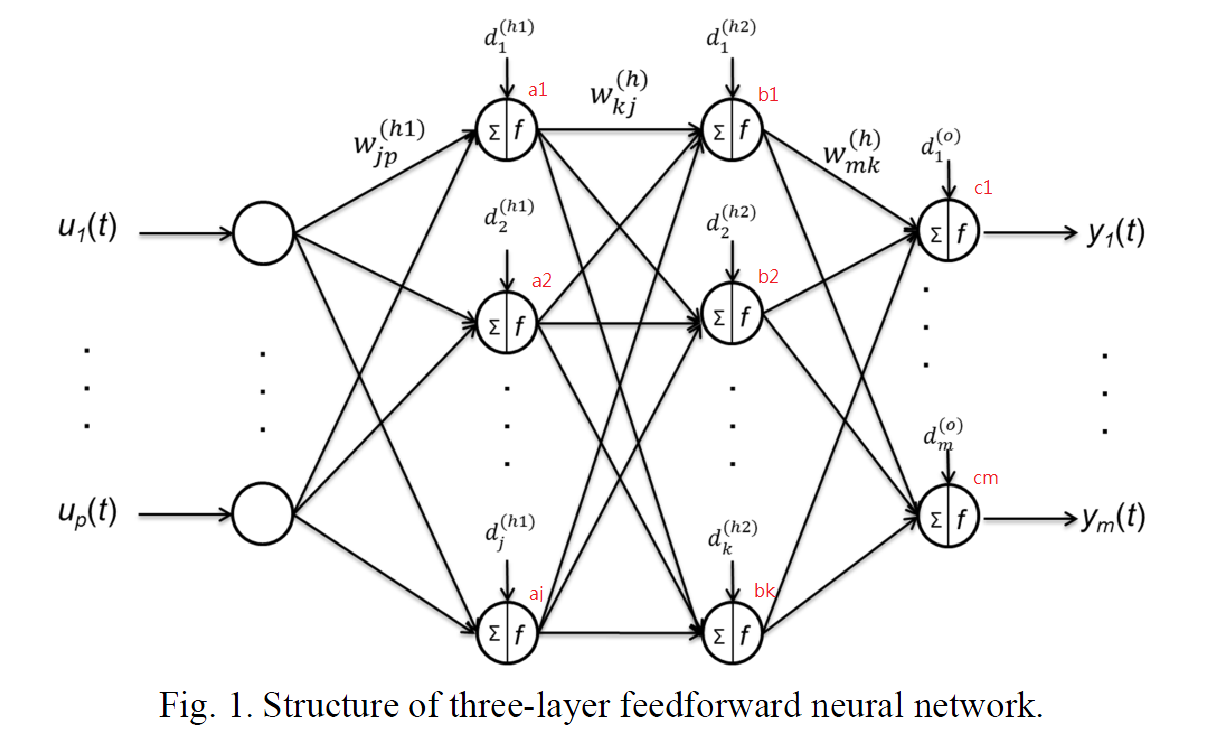
\includegraphics[scale=0.5]{hw2}

\begin{enumerate}
	\vspace{0.7cm}
	\item Forward path:
\vspace{0.5cm}
\\	
	$a_j=\sum\limits_{\alpha=1 \sim j,\  \beta=1 \sim p}
w_{\alpha\beta}^{(h1)} \times u_\beta(t)+d_\alpha^{(h1)} $
\vspace{0.5cm}
\\
	$Y_{a_j}=f(a_j)$
\vspace{0.5cm}
\\
	$b_k=\sum\limits_{\alpha=1 \sim k,\  \beta=1 \sim j}
w_{\alpha\beta}^{(h2)} \times Y_{a_\beta}+d_\alpha^{(h2)} $
\vspace{0.5cm}
\\
	$Y_{b_k}=g(b_k)$
\vspace{0.5cm}
\\
	$y_m(t)=c_m=\sum\limits_{\alpha=1 \sim m,\  \beta=1 \sim k}
	w_{\alpha\beta}^{(h3)} \times y_{b_\beta}+d_\alpha^{(o)} $
\\[0.5cm]
\noindent\rule{\textwidth}{1pt}
\\[0.5cm]
$E_m(t)=\frac{1}{2}e_m^2(t)
\\[0.5cm]
e_m(t)=d_m(t)-y_m(t)
$
\\[0.3cm]
for part1 $d_m(t)$ is composed of 1 and 0
\newpage
\item Backward propagation
\begin{enumerate}
	\item Update rule for the weights of the output neurons:
\vspace{0.5cm}
\\
$
	\begin{aligned}
	w_{mk}^{(h_3)}(t+1) & =w_{mk}^{(h_3)}(t)+\Delta w_{mk}(t)
\\[0.5cm]
	& =	w_{mk}^{(h_3)}(t)-\eta\frac{\partial E_m(t)}{\partial w_{mk}^{(h_3)}(t)}
\\[0.5cm]
	& = w_{mk}^{(h_3)}(t)-\eta\frac{\partial E_m(t)}{\partial e_{m}(t)}
	\frac{\partial e_{m}(t)}{\partial y_m(t)}
	\frac{\partial y_m(t)}{\partial c_{m}(t)}
	\frac{\partial c_m(t)}{\partial w_{mk}^{(h_3)}(t)}
\\[0.5cm]
	& = w_{mk}^{(h_3)}(t)-\eta(d_m(t)-y_m(t))(-1)(1)(Y_{b_k}(t))
\\[0.5cm]
	& = w_{mk}^{(h_3)}(t)+\eta(d_m(t)-y_m(t))(Y_{b_k}(t))	
	\end{aligned}
$
	\item Update rule for the biases of the output neurons:
\vspace{0.5cm}
\\
$
\begin{aligned}
d_{m}^{(o)}(t+1) & =d_{m}^{(o)}(t)+\Delta d_{m}(t)
\\[0.5cm]
& =d_{m}^{(o)}(t)-\eta\frac{\partial E_m(t)}{\partial d_{m}^{(o)}(t)}
\\[0.5cm]
& =d_{m}^{(o)}(t)-\eta\frac{\partial E_m(t)}{\partial e_{j}(t)}
\frac{\partial e_{m}(t)}{\partial y_m(t)}
\frac{\partial y_m(t)}{\partial c_{m}(t)}
\frac{\partial c_m(t)}{\partial d_{m}^{(o)}(t)}
\\[0.5cm]
& =d_{m}^{(o)}(t)-\eta(d_m(t)-y_m(t))(-1)(1)(1)
\\[0.5cm]
& =d_{m}^{(o)}(t)+\eta(d_m(t)-y_m(t))
\end{aligned}
$
\newpage

	\item Update rule for the weights of the second hidden neurons:
\vspace{0.5cm}
\\
$
\begin{aligned}
w_{kj}^{(h_2)}(t+1) & =w_{kj}^{(h_2)}(t)+\Delta w_{kj}(t)
\\[0.5cm]
& =	w_{kj}^{(h_2)}(t)-\eta\frac{\partial E_m(t)}{\partial w_{kj}^{(h_2)}(t)}
\\[0.5cm]
& = w_{kj}^{(h_2)}(t)-\eta\frac{\partial E_m(t)}{\partial e_{m}(t)}
\frac{\partial e_{m}(t)}{\partial y_m(t)}
\frac{\partial y_m(t)}{\partial c_{m}(t)}
\frac{\partial c_m(t)}{\partial Y_{b_k}(t)}
\frac{\partial Y_{b_k}(t)}{\partial b_k(t)}
\frac{\partial b_k(t)}{\partial w_{kj}^{(h_2)}(t)}
\\[0.5cm]
& = w_{kj}^{(h_2)}(t)-\eta\sum_m(d_m(t)-y_m(t))(-1)(1)(w_{mk}^{(h_3)}(t))g'(b_k(t))(Y_{a_j}(t))
\\[0.5cm]
& = w_{kj}^{(h_2)}(t)+\eta\sum_m(d_m(t)-y_m(t))(w_{mk}^{(h_3)}(t))g'(b_k(t))(Y_{a_j}(t))
\end{aligned}
$

	\item Update rule for the biases of the second hidden neurons:
\vspace{0.5cm}
\\
$
\begin{aligned}
d_{k}^{(h_2)}(t+1) & =d_{k}^{(h_2)}(t)+\Delta d_{k}(t)
\\[0.5cm]
& =d_{k}^{(h_2)}(t)-\eta\frac{\partial E_m(t)}{\partial d_{k}^{(h_2)}(t)}
\\[0.5cm]
& =d_{k}^{(h_2)}(t)-\eta\frac{\partial E_m(t)}{\partial e_{j}(t)}
\frac{\partial e_{m}(t)}{\partial y_m(t)}
\frac{\partial y_m(t)}{\partial c_{m}(t)}
\frac{\partial c_m(t)}{\partial Y_{b_k}(t)}
\frac{\partial Y_{b_k}(t)}{\partial b_k(t)}
\frac{\partial b_k(t)}{\partial d_j^{(h_1)}(t)}
\\[0.5cm]
& =d_{k}^{(h_2)}(t)-\eta\sum_m(d_m(t)-y_m(t))(-1)(1)(w_{mk}^{(h_3)}(t))g'(b_k(t))(1)
\\[0.5cm]
& =d_{k}^{(h_2)}(t)+\eta\sum_m(d_m(t)-y_m(t))(w_{mk}^{(h_3)}(t))g'(b_k(t))
\end{aligned}
$
\newpage


\item Update rule for the weights of the first hidden neurons:
\vspace{0.5cm}
\\
$
\begin{aligned}
w_{jp}^{(h_1)}(t+1) & =w_{jp}^{(h_1)}(t)+\Delta w_{jp}(t)
\\[0.5cm]
& =w_{jp}^{(h_1)}(t)-\eta\frac{\partial E_m(t)}{\partial w_{jp}^{(h_1)}(t)}
\\[0.5cm]
& = w_{jp}^{(h_1)}(t)-\eta\frac{\partial E_m(t)}{\partial e_{m}(t)}
\frac{\partial e_{m}(t)}{\partial y_m(t)}
\frac{\partial y_m(t)}{\partial c_{m}(t)}
\frac{\partial c_m(t)}{\partial Y_{b_k}(t)}
\frac{\partial Y_{b_k}(t)}{\partial b_k(t)}
\frac{\partial b_k(t)}{\partial Y_{aj}(t)}
\\[0.5cm]
&\ \hspace{9cm}
\frac{\partial Y_{aj}(t)}{\partial a_j(t)}
\frac{\partial a_{j}(t)}{\partial w_{jp}^{(h_1)}(t)}
\\[0.5cm]
& = w_{jp}^{(h_1)}(t)-\eta\sum_k\sum_m(d_m(t)-y_m(t))(-1)(1)(w_{mk}^{(h_3)}(t))
g'(b_k(t))
\\[0.5cm]
&\ \hspace{8cm}
(w_{kj}^{(h_2)}(t))f'(a_j(t))(u_p(t))
\\[0.5cm]
& = w_{jp}^{(h_1)}(t)+\eta\sum_k\sum_m(d_m(t)-y_m(t))(w_{mk}^{(h_3)}(t))
g'(b_k(t))(w_{kj}^{(h_2)}(t))
\\[0.5cm]
&\ \hspace{10cm}
f'(a_j(t))(u_p(t))
\end{aligned}
$

\newpage
\item Update rule for the biases of the first hidden neurons:
\vspace{0.5cm}
\\
$
\begin{aligned}
d_{j}^{(h_1)}(t+1) & =d_{j}^{(h_1)}(t)+\Delta d_{j}(t)
\\[0.5cm]
& =d_{j}^{(h_1)}(t)-\eta\frac{\partial E_m(t)}{\partial d_{j}^{(h_1)}(t)}
\\[0.5cm]
& =d_{j}^{(h_1)}(t)-\eta\frac{\partial E_m(t)}{\partial e_{j}(t)}
\frac{\partial e_{m}(t)}{\partial y_m(t)}
\frac{\partial y_m(t)}{\partial c_{m}(t)}
\frac{\partial c_m(t)}{\partial Y_{b_k}(t)}
\frac{\partial Y_{b_k}(t)}{\partial b_k(t)}
\frac{\partial b_k(t)}{\partial Y_{a_j}(t)}
\\[0.5cm]
&\ \hspace{9cm}
\frac{\partial Y_{aj}(t)}{\partial a_j(t)}
\frac{\partial a_{j}(t)}{\partial d_{j}^{(h_1)}(t)}
\\[0.5cm]
& =d_{j}^{(h_1)}(t)-\eta\sum_k\sum_m(d_m(t)-y_m(t))(-1)(1)(w_{mk}^{(h_3)}(t))
g'(b_k(t))
\\[0.5cm]
&\ \hspace{9cm}
(w_{kj}^{(h_2)}(t))f'(a_j(t))(1)
\\[0.5cm]
\\[0.5cm]
& =d_{j}^{(h_1)}(t)+\eta\sum_k\sum_m(d_m(t)-y_m(t))(w_{mk}^{(h_3)}(t))
g'(b_k(t))(w_{kj}^{(h_2)}(t))f'(a_j(t))
\end{aligned}
$
\\[0.5cm]
\noindent\rule{\textwidth}{1pt}
\\[0.5cm]
In this homework, we will use
\begin{enumerate}
\item hyperbolic tangent functions for all the hidden layers
\item sigmoid functions for all the hidden layers
\item hyperbolic tangent functions for the first hidden layer and sigmoid functions for the second layer
\end{enumerate}
as the activation function $f()$ and $g()$ to evaluate the network performance.

\end{enumerate}
\end{enumerate}
\newpage

\title{\large \bf  Part1: classification}
\\
\begin{enumerate}
	%%%%%%%%%%%%%%%%%%%%%%%%%%%%%%%%%%%%
	\item Iris 
	\begin{enumerate}
	\item topologies (structures) of the networks: \\
	input layer node: 4 \\
	first hidden layer node: 2 \\
	second hidden layer node: 3 \\
	output layer node: 3\\
	all layers are fully connected
	\item best three results out of 10 trials using different initializations:
	\begin{enumerate}
		\item hyperbolic tangent functions for all the hidden layers:
		\\
		learning rate = 0.1 \\
		epoch = 20
		\begin{enumerate}
\item accuracy = 100\%\\\
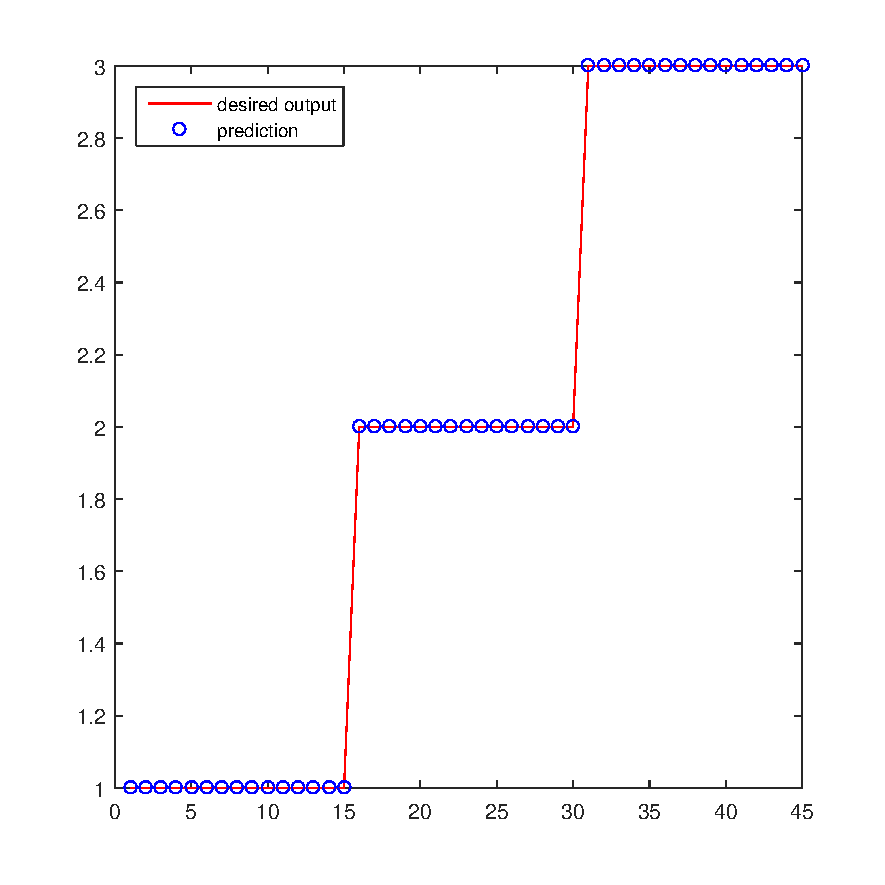
\includegraphics[scale=0.6]{irishh1}
\newpage	
\item accuracy = 100\%\\\
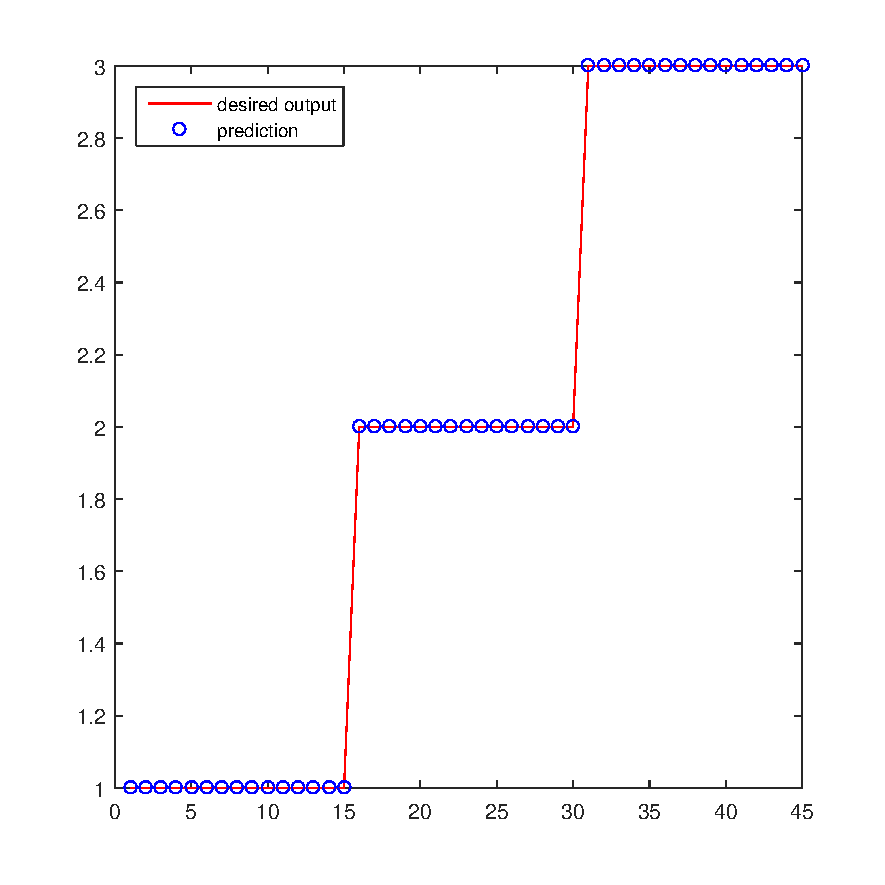
\includegraphics[scale=0.6]{irishh1}	
\item accuracy = 100\%\\\
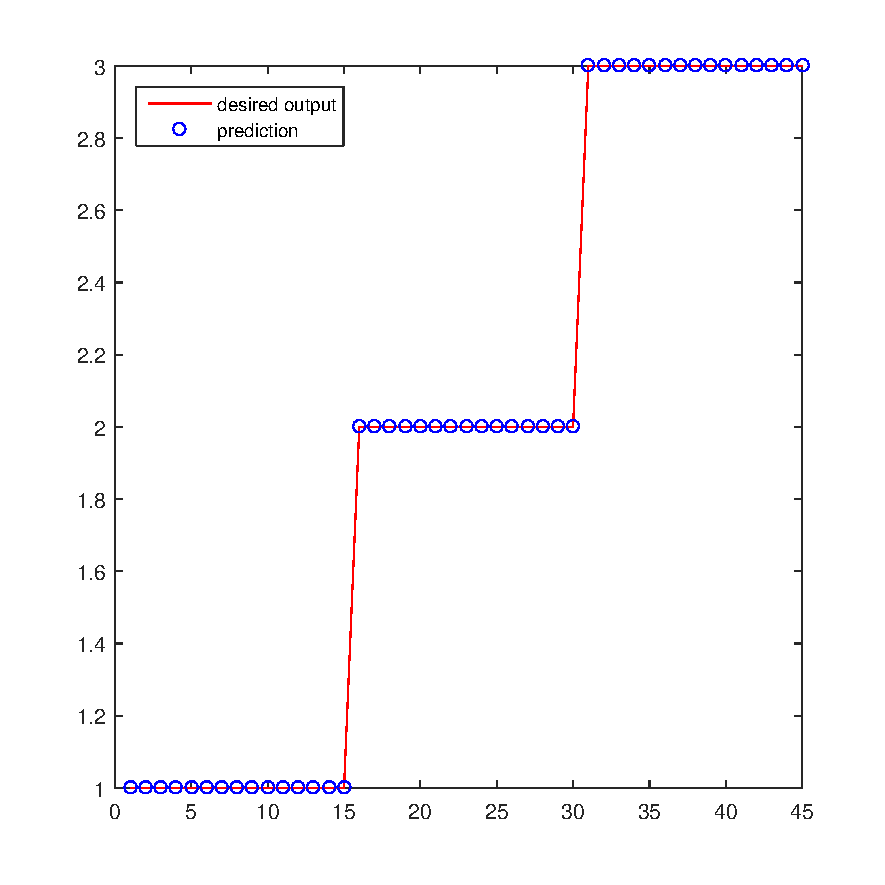
\includegraphics[scale=0.6]{irishh1}		
\newpage	
		\end{enumerate}
	\item sigmoid functions for all the hidden layers:
	\\
	learning rate = 0.1 \\
	epoch = 50
	\begin{enumerate}
		\item accuracy = 97.8\%\ \\
		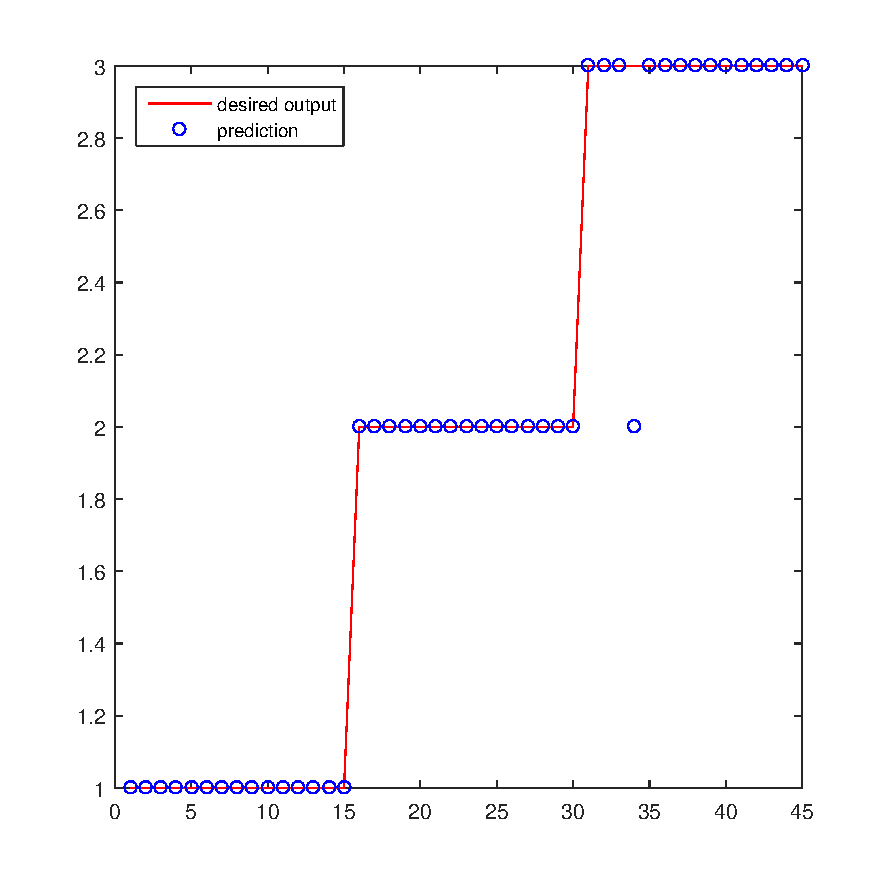
\includegraphics[scale=0.6]{irisss1}
		\newpage	
		\item accuracy = 97.8\%\ \\
		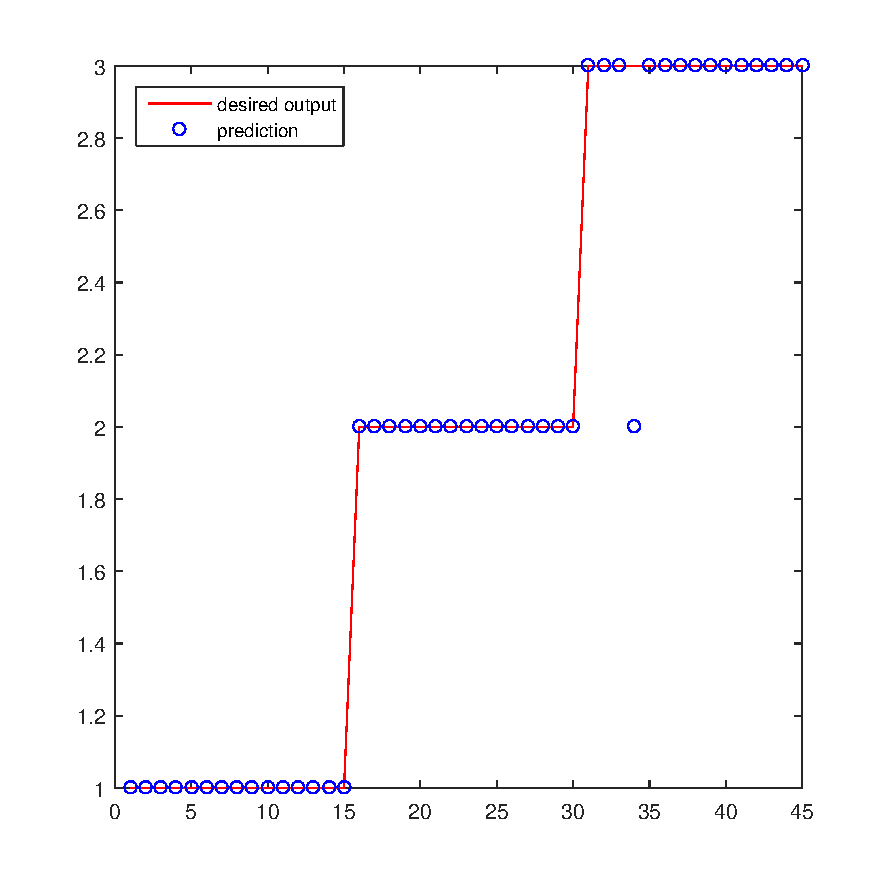
\includegraphics[scale=0.6]{irisss1}	
		\item accuracy = 97.8\%\ \\
		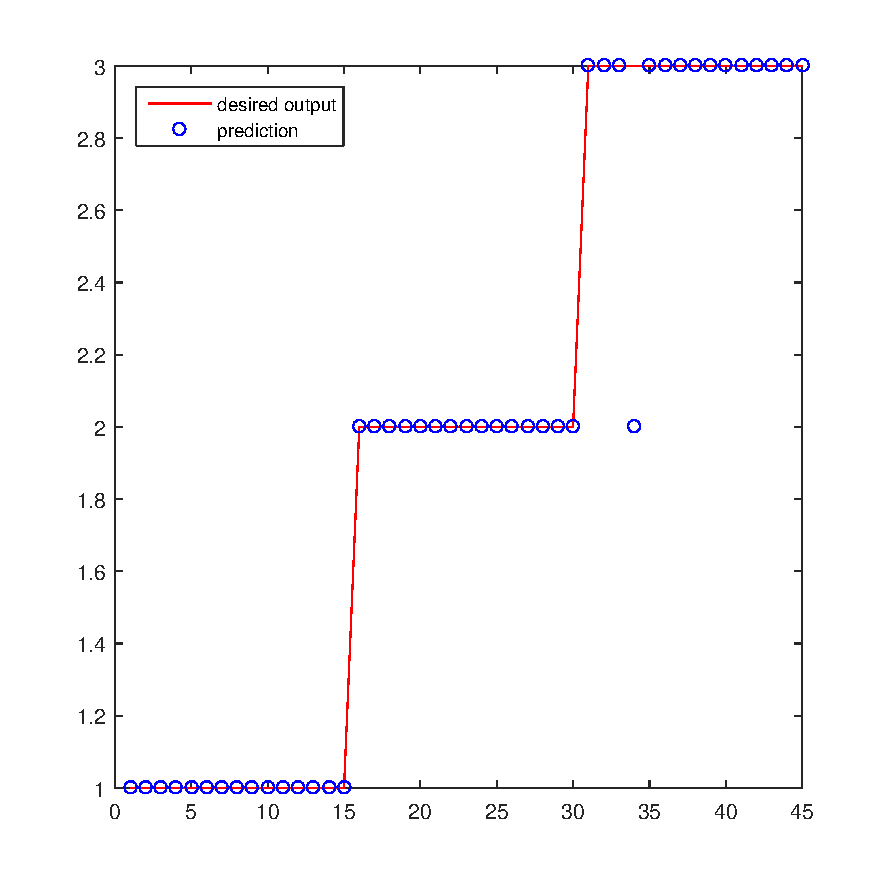
\includegraphics[scale=0.6]{irisss1}		
		\newpage	
	\end{enumerate}
\item hyperbolic tangent functions for the first hidden layer and sigmoid functions for the second layer:
\\
learning rate = 0.1 \\
epoch = 20
\begin{enumerate}
	\item accuracy = 100\%\ \\
	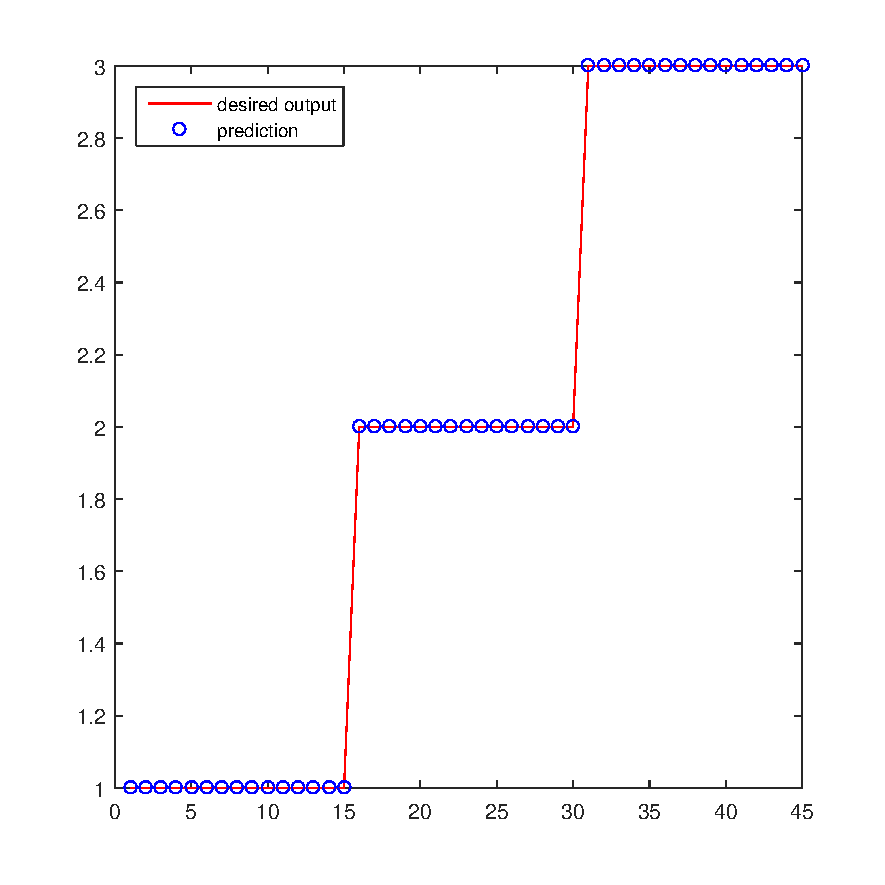
\includegraphics[scale=0.6]{irishs1}
	\newpage	
	\item accuracy = 100\%\ \\
	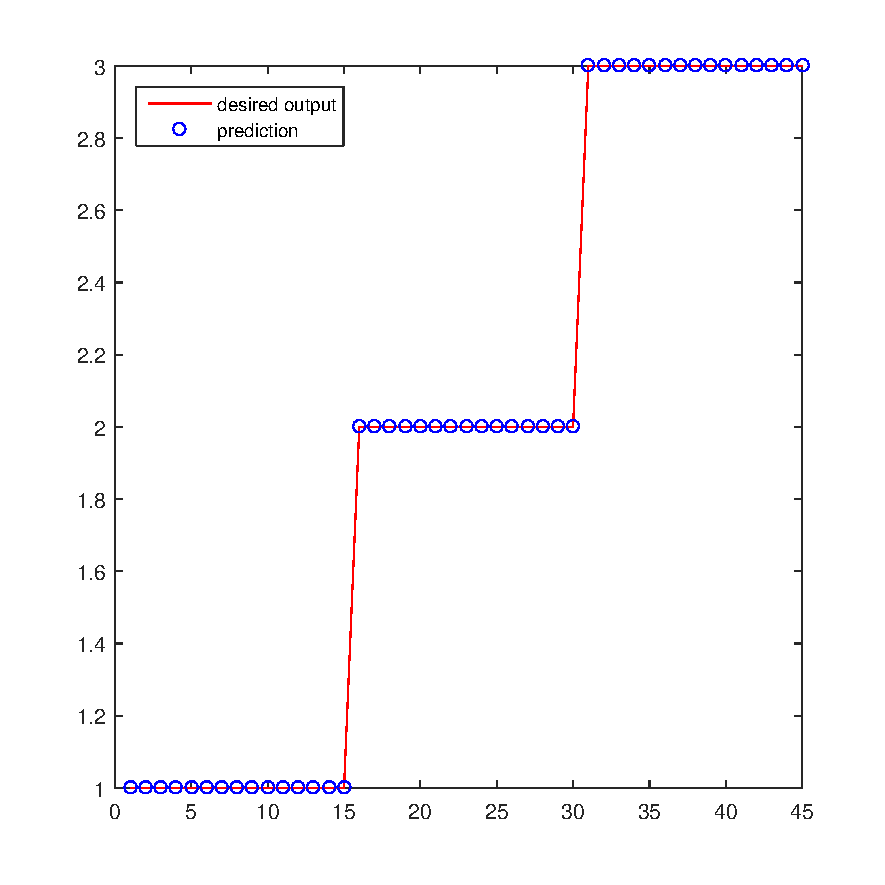
\includegraphics[scale=0.6]{irishs1}	
	\item accuracy = 100\%\ \\
	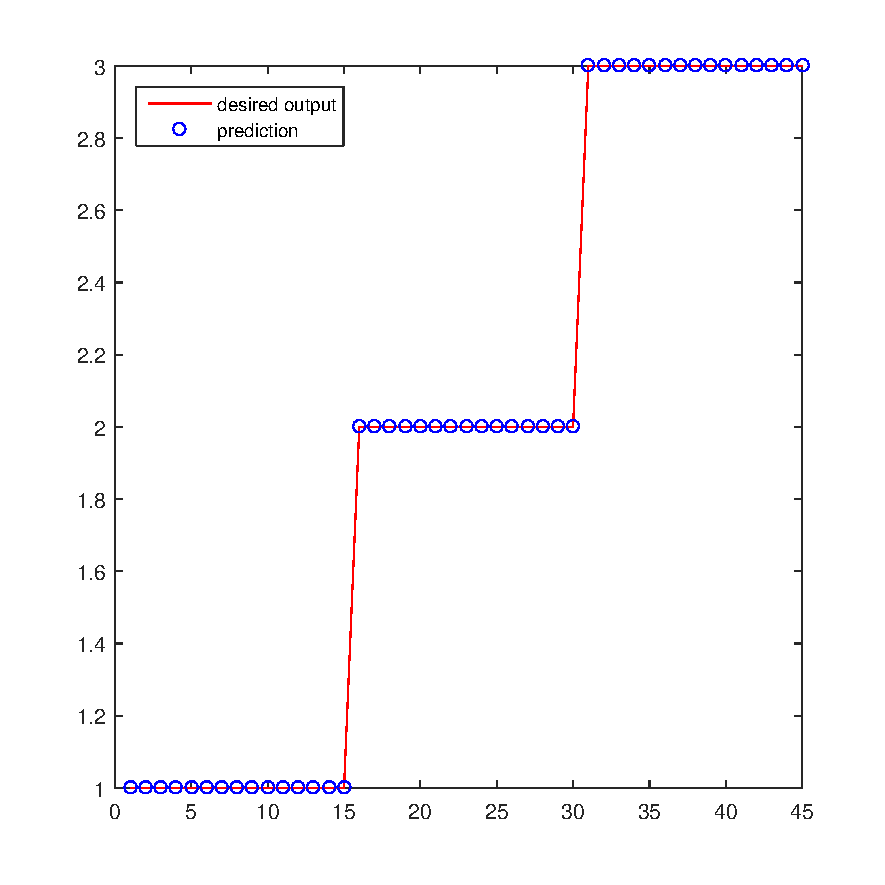
\includegraphics[scale=0.6]{irishs1}		
	\newpage	
\end{enumerate}
	\end{enumerate}

\item For the random weight assignment, use the same initial weights that you obtain the best classification result to compare the learning curves with different learning rates:
\\
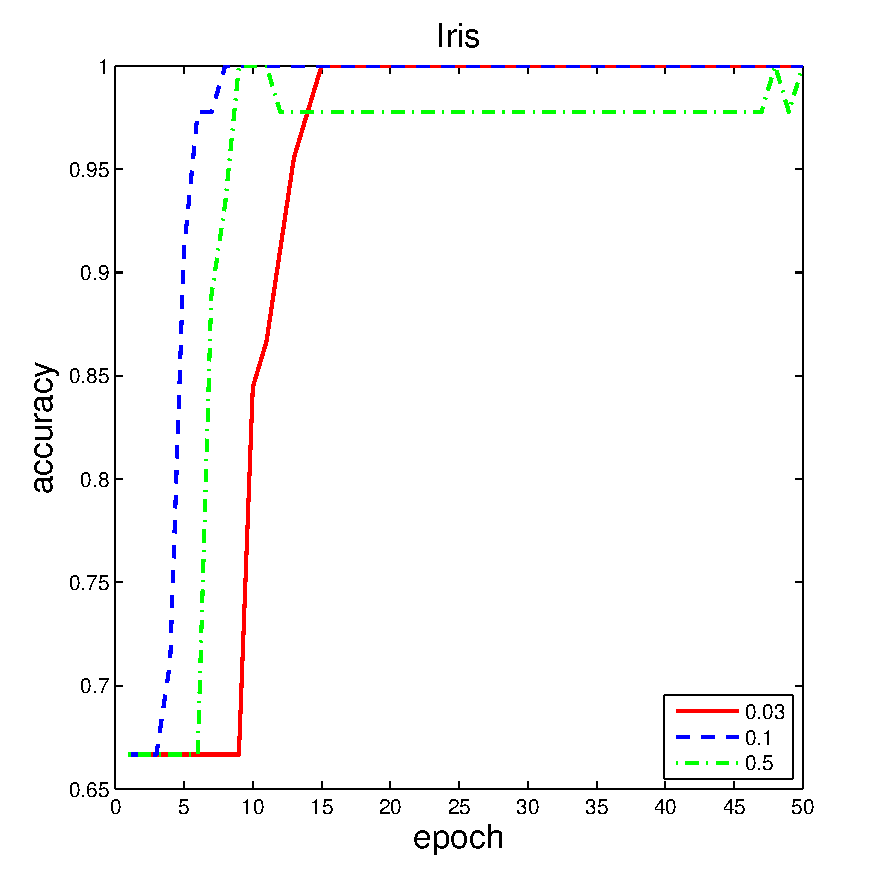
\includegraphics[scale=0.7]{iriscurve}

	\end{enumerate}
\newpage
%%%%%%%%%%%%%%%%%%%%%%%%%%%%%%%%%%%%%%%%%%%%%%%
\item Wine
\begin{enumerate}
	\item topologies (structures) of the networks: \\
	input layer node: 13 \\
	first hidden layer node: 4 \\
	second hidden layer node: 2 \\
	output layer node: 3\\
	all layers are fully connected
	\item best three results out of 10 trials using different initializations:
	\begin{enumerate}
		\item hyperbolic tangent functions for all the hidden layers:
		\\
		learning rate = 0.1 \\
		epoch = 30
		\begin{enumerate}
			\item accuracy = 100\%\\\
			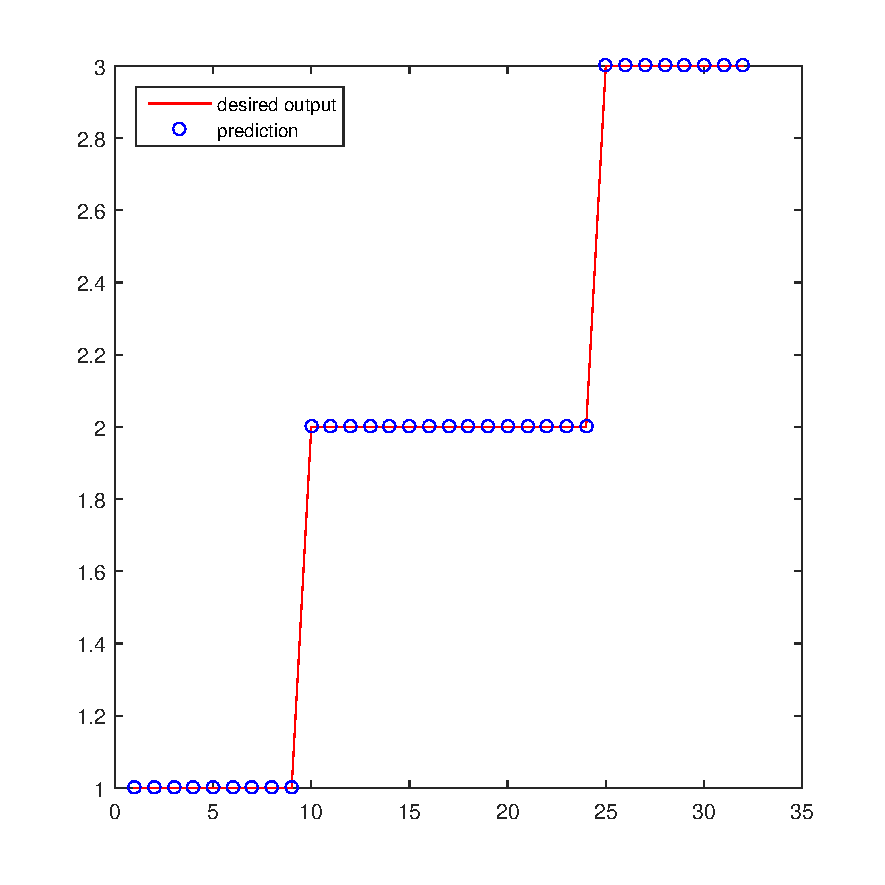
\includegraphics[scale=0.6]{winehh1}
			\newpage	
			\item accuracy = 100\%\\\
			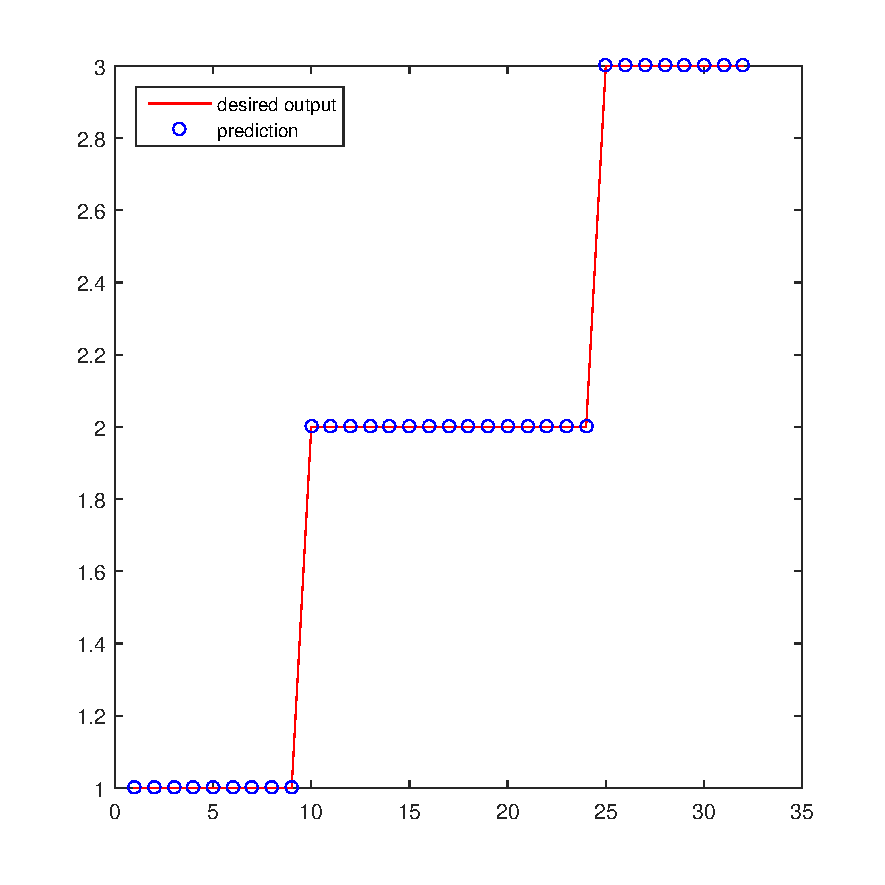
\includegraphics[scale=0.6]{winehh1}	
			\item accuracy = 100\%\\\
			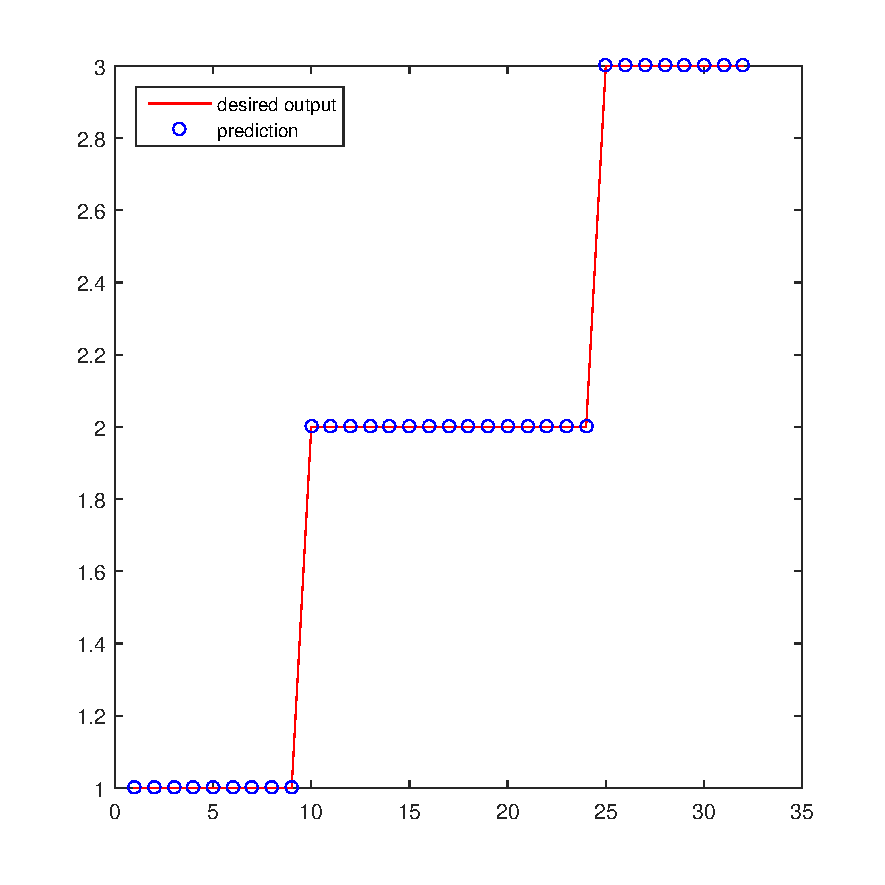
\includegraphics[scale=0.6]{winehh1}		
			\newpage	
		\end{enumerate}
		\item sigmoid functions for all the hidden layers:
		\\
		learning rate = 0.1 \\
		epoch = 30
		\begin{enumerate}
			\item accuracy = 96.9\%\ \\
			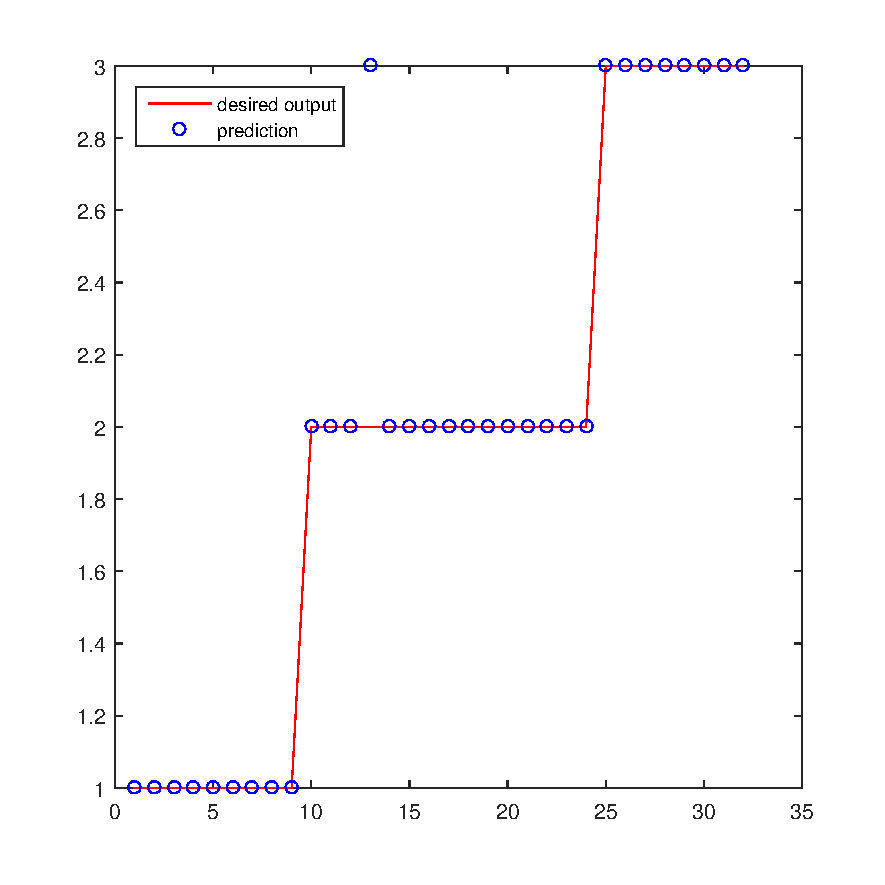
\includegraphics[scale=0.6]{winess1}
			\newpage	
			\item accuracy = 96.9\%\ \\
			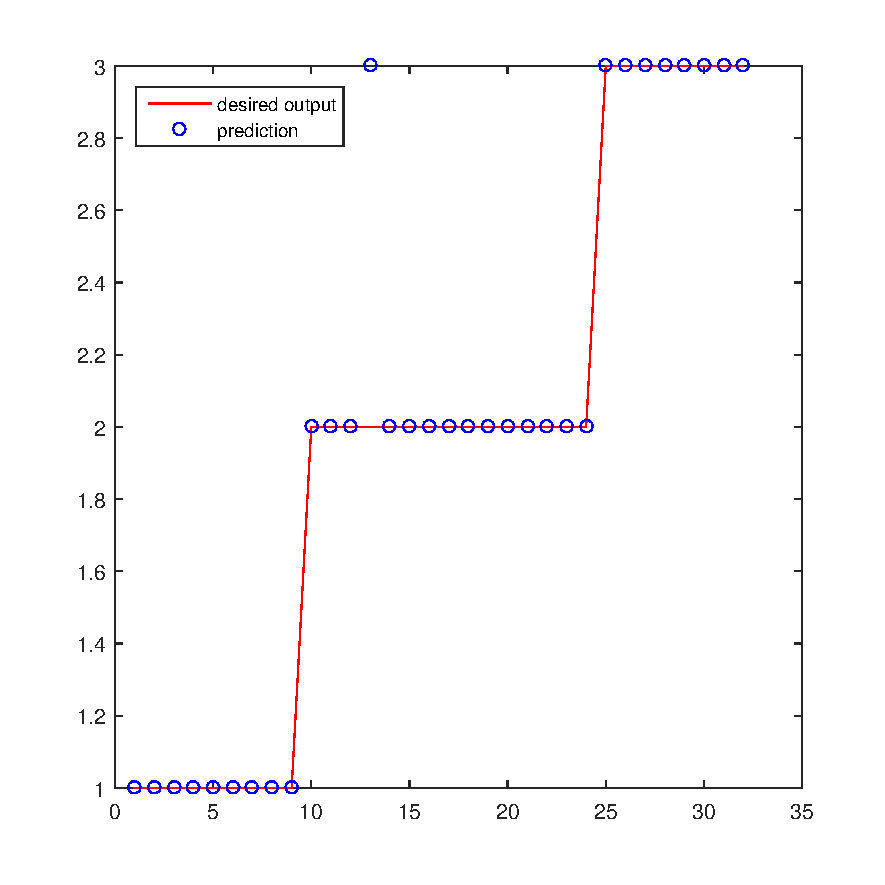
\includegraphics[scale=0.6]{winess1}	
			\item accuracy = 96.9\%\ \\
			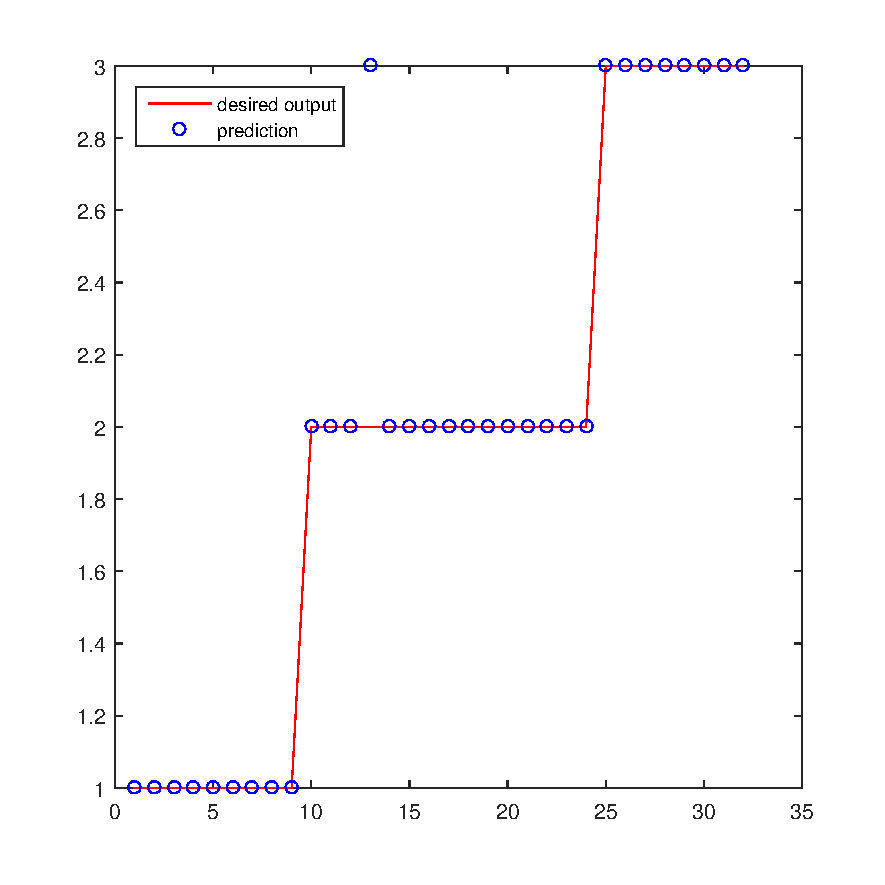
\includegraphics[scale=0.6]{winess1}		
			\newpage	
		\end{enumerate}
		\item hyperbolic tangent functions for the first hidden layer and sigmoid functions for the second layer:
		\\
		learning rate = 0.1 \\
		epoch = 30
		\begin{enumerate}
			\item accuracy = 100\%\ \\
			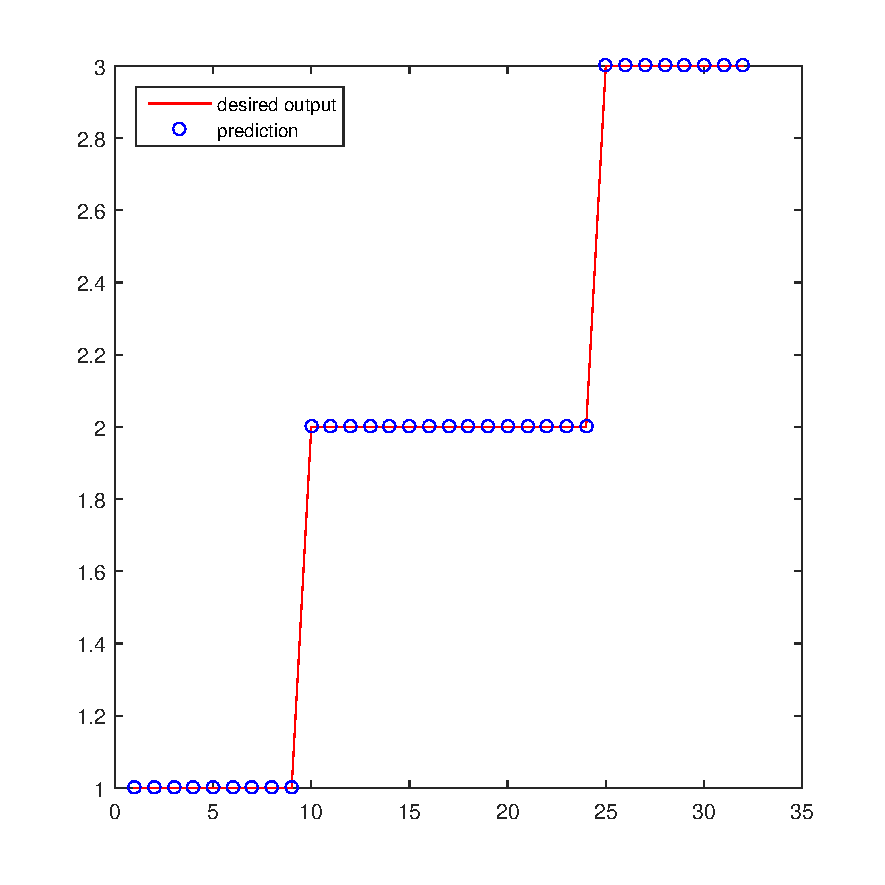
\includegraphics[scale=0.6]{winehs1}
			\newpage	
			\item accuracy = 100\%\ \\
			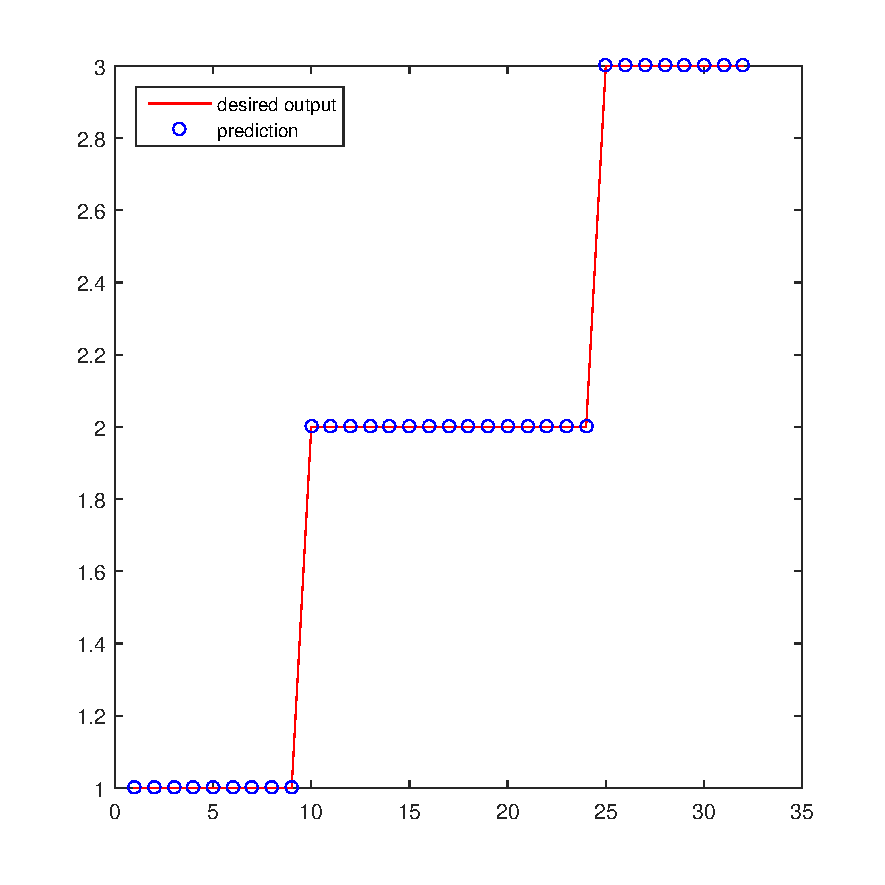
\includegraphics[scale=0.6]{winehs1}	
			\item accuracy = 100\%\ \\
			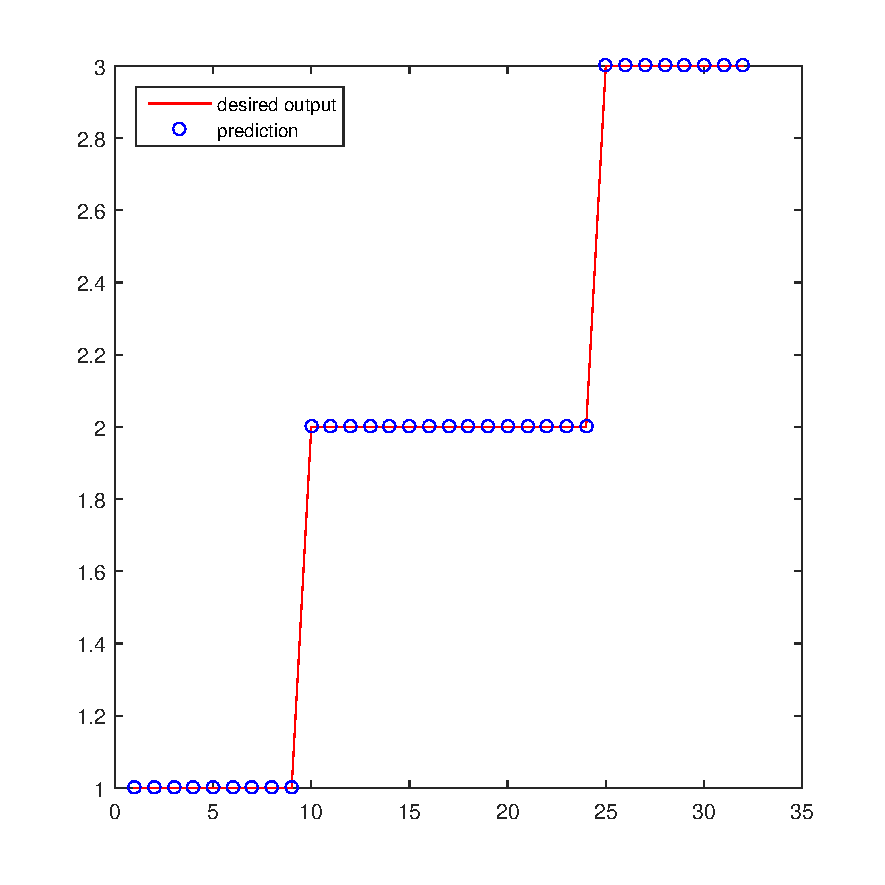
\includegraphics[scale=0.6]{winehs1}		
			\newpage	
		\end{enumerate}
	\end{enumerate}
	
	\item For the random weight assignment, use the same initial weights that you obtain the best classification result to compare the learning curves with different learning rates:
	\\
	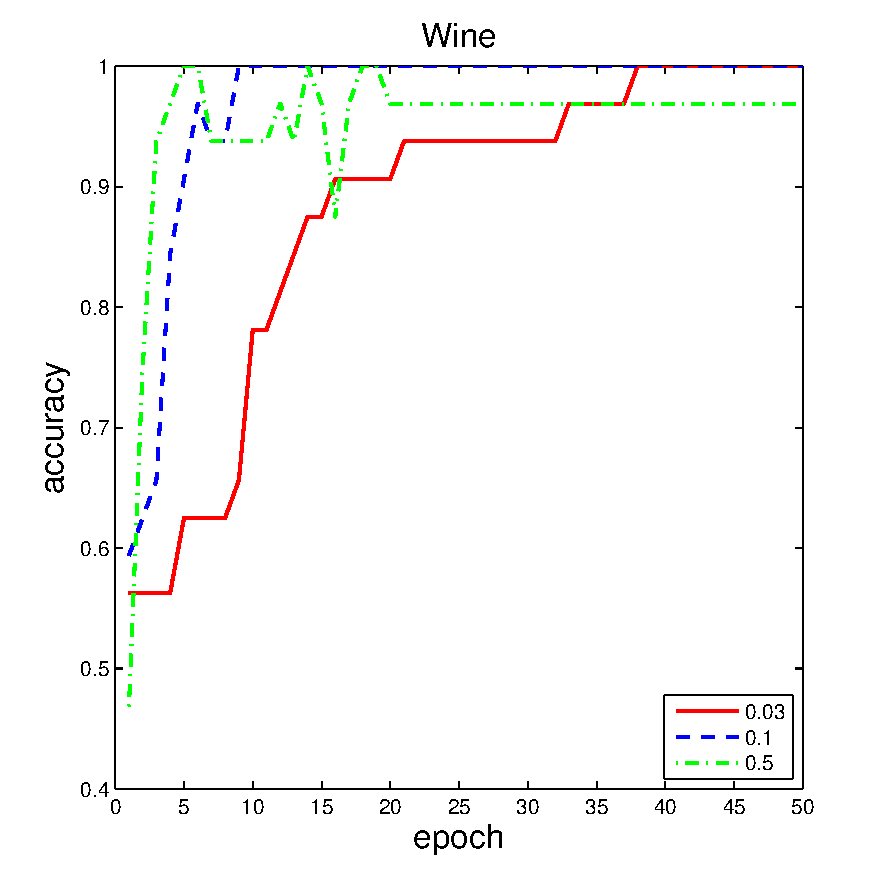
\includegraphics[scale=0.7]{winecurve}
\end{enumerate}
\newpage
%%%%%%%%%%%%%%%%%%%%%%%%%%%%%%%%%%%%%%%%%%%%%%%%%%%%%%%%
\item Breast Cancer Wisconsin 
\begin{enumerate}
	\item topologies (structures) of the networks: \\
	input layer node: 9 \\
	first hidden layer node: 3 \\
	second hidden layer node: 3 \\
	output layer node: 2\\
	all layers are fully connected
	\item best three results out of 10 trials using different initializations:
	\begin{enumerate}
		\item hyperbolic tangent functions for all the hidden layers:
		\\
		learning rate = 0.1 \\
		epoch = 15
		\begin{enumerate}
			\item accuracy = 98.4\%\\\
			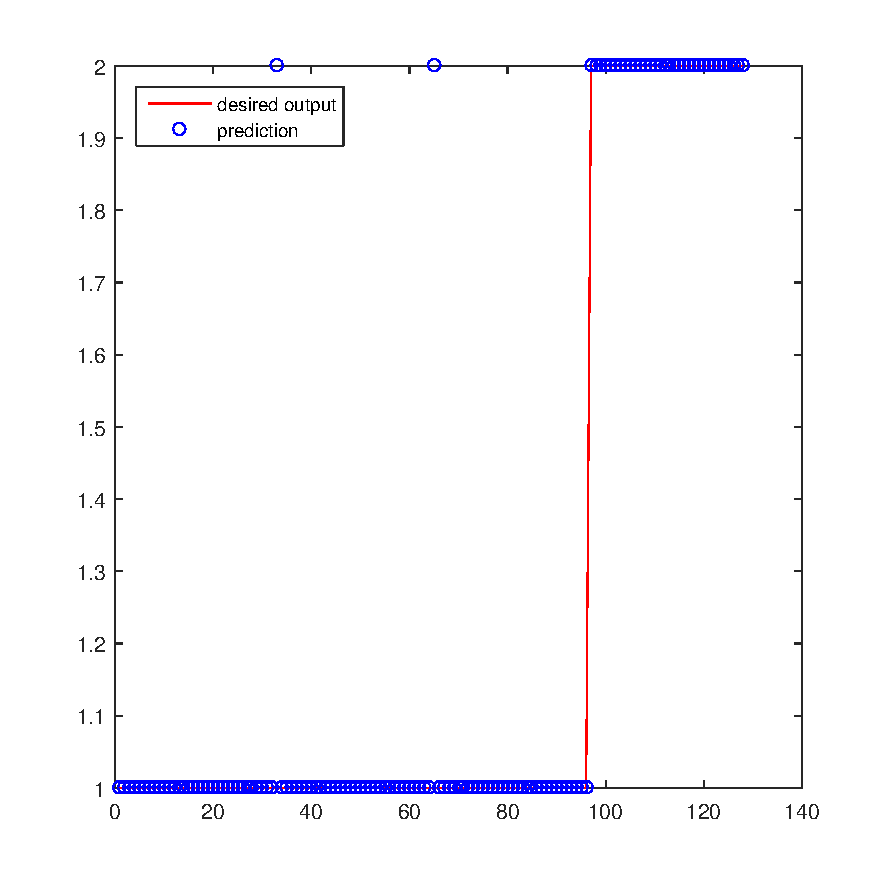
\includegraphics[scale=0.6]{breasthh1}
			\newpage	
			\item accuracy = 98.4\%\\\
			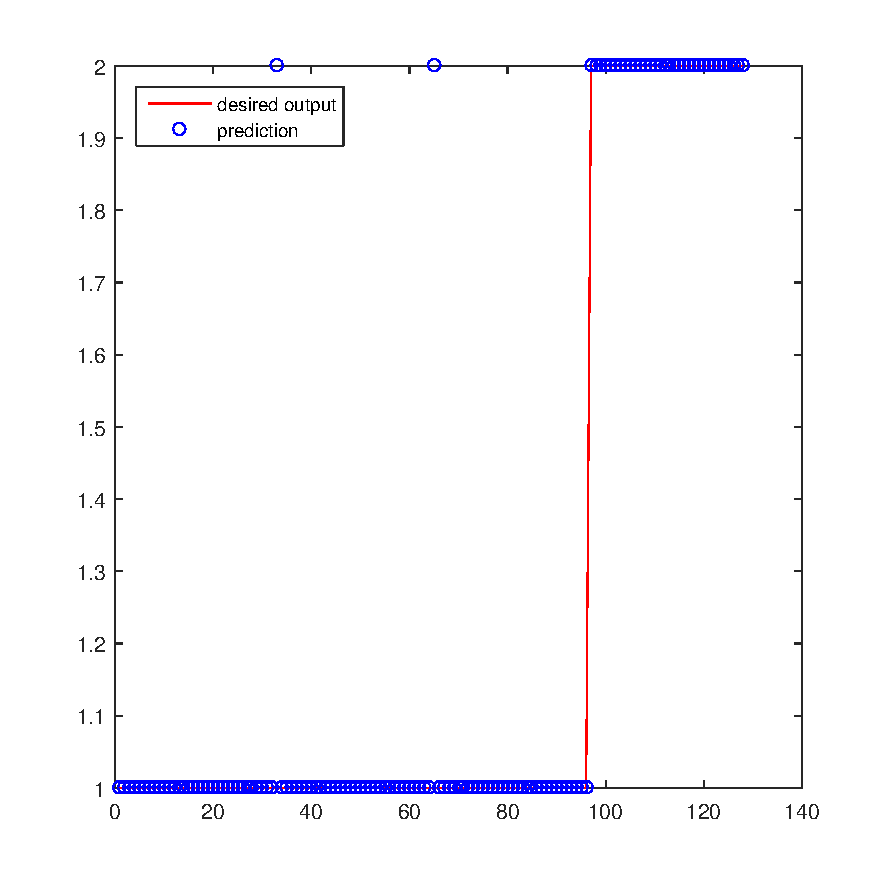
\includegraphics[scale=0.6]{breasthh1}	
			\item accuracy = 98.4\%\\\
			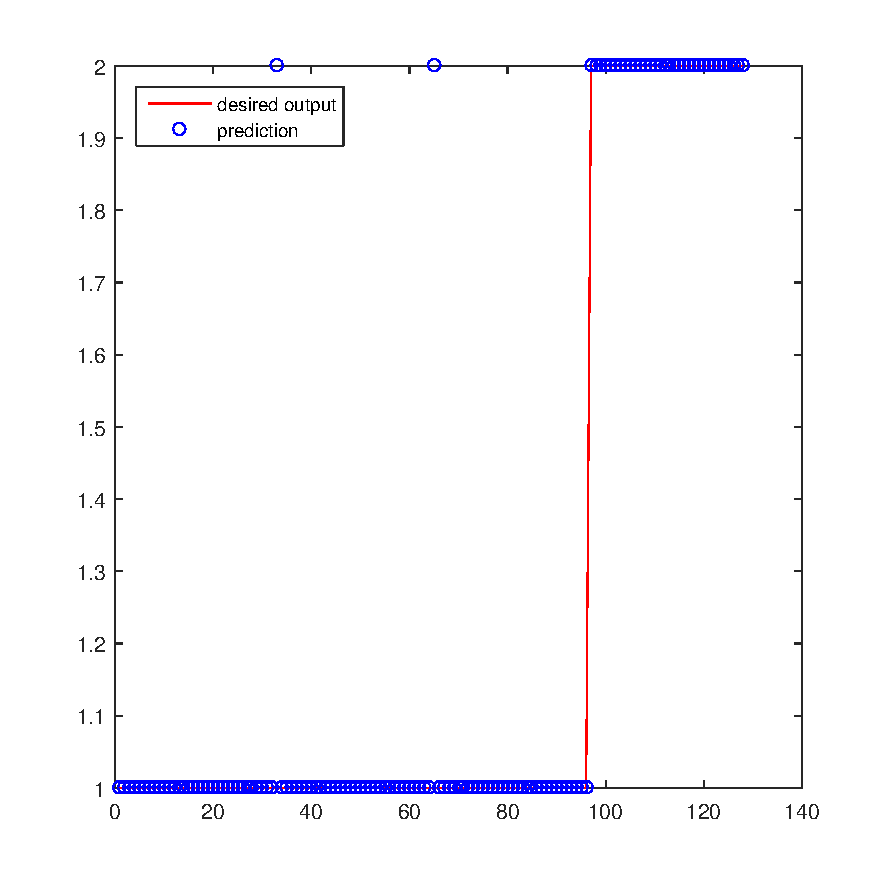
\includegraphics[scale=0.6]{breasthh1}		
			\newpage	
		\end{enumerate}
		\item sigmoid functions for all the hidden layers:
		\\
		learning rate = 0.1 \\
		epoch = 20
		\begin{enumerate}
			\item accuracy = 97.7\%\ \\
			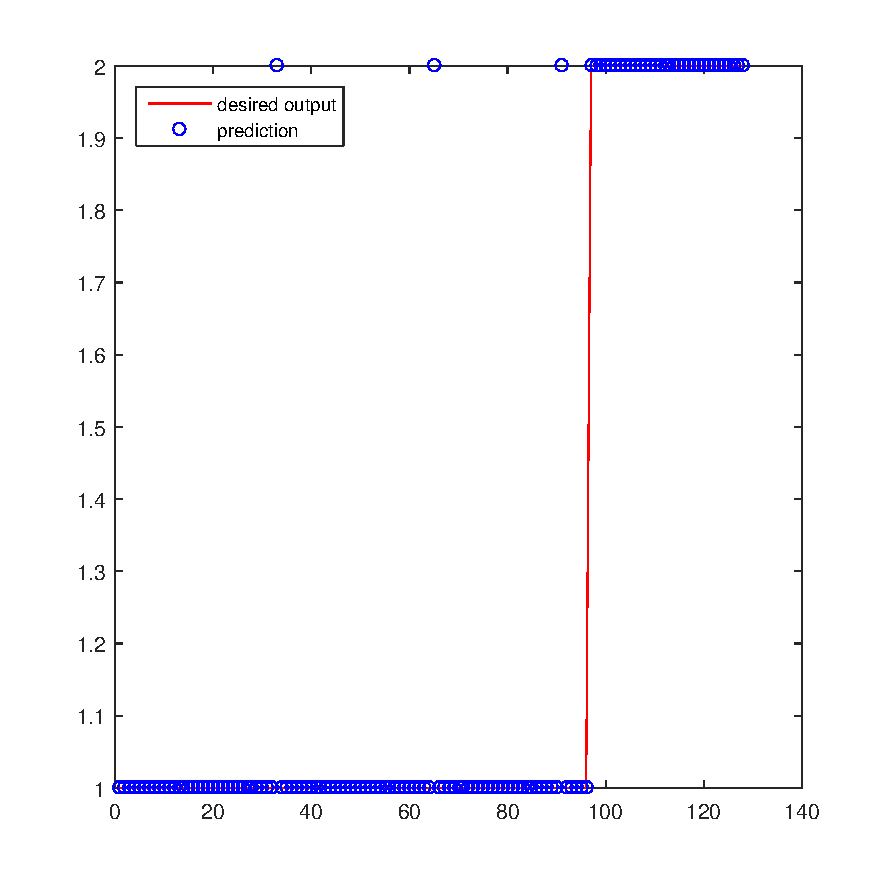
\includegraphics[scale=0.6]{breastss1}
			\newpage	
			\item accuracy = 97.7\%\ \\
			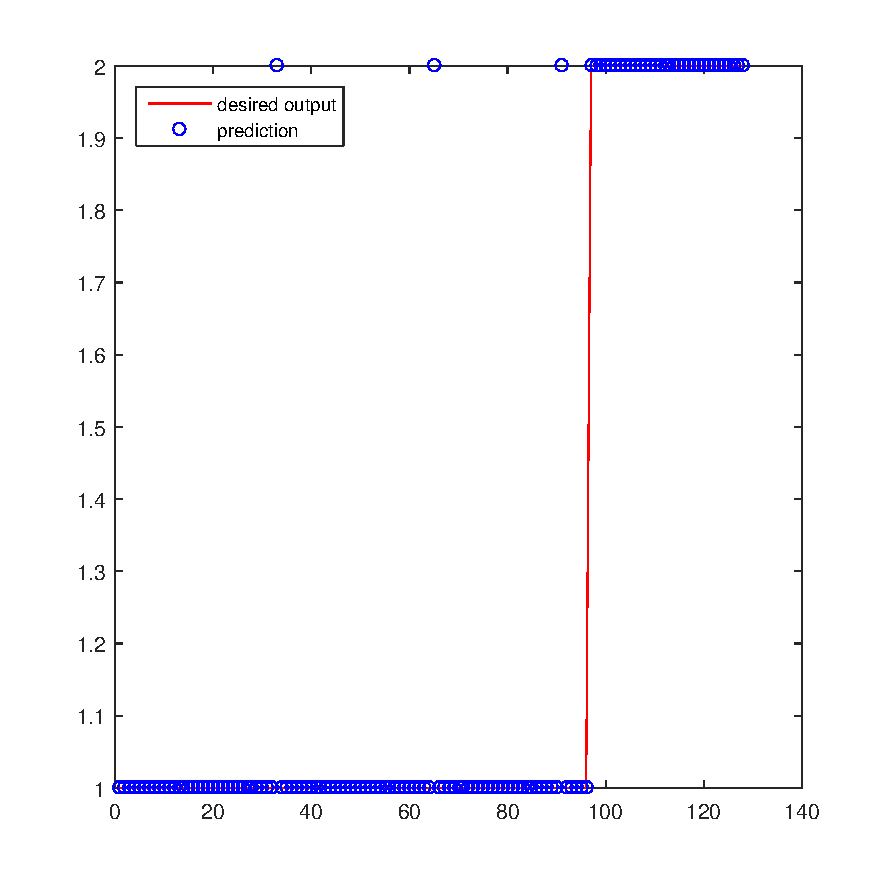
\includegraphics[scale=0.6]{breastss1}	
			\item accuracy = 97.7\%\ \\
			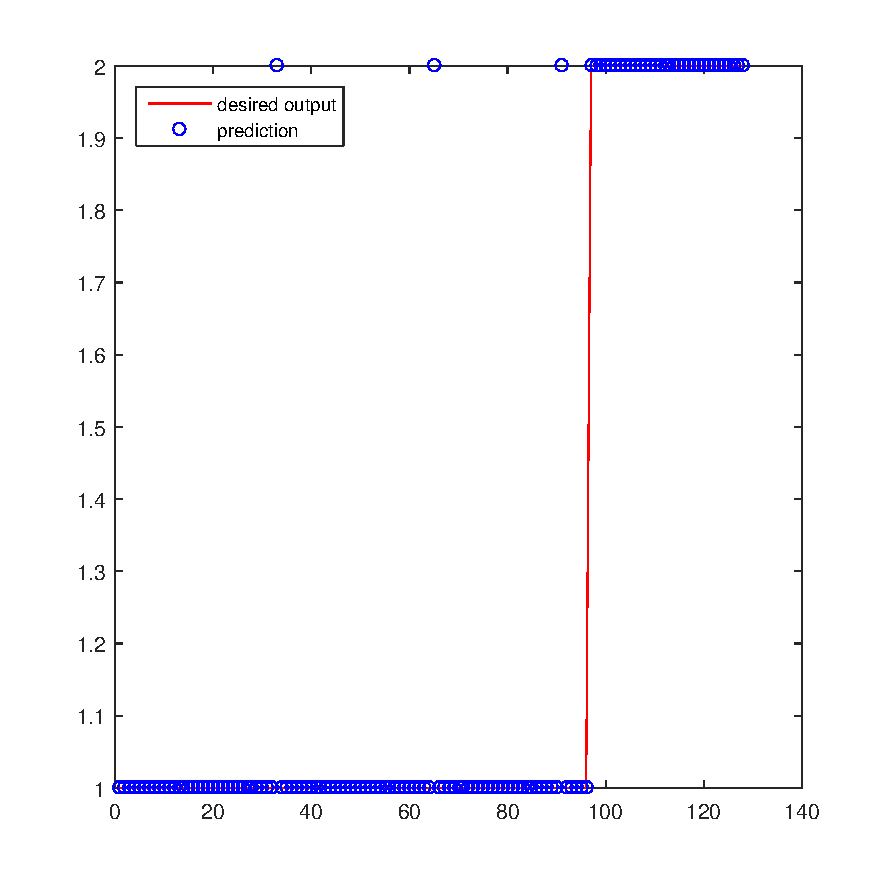
\includegraphics[scale=0.6]{breastss1}		
			\newpage	
		\end{enumerate}
		\item hyperbolic tangent functions for the first hidden layer and sigmoid functions for the second layer:
		\\
		learning rate = 0.1 \\
		epoch = 20
		\begin{enumerate}
			\item accuracy = 98.4\%\ \\
			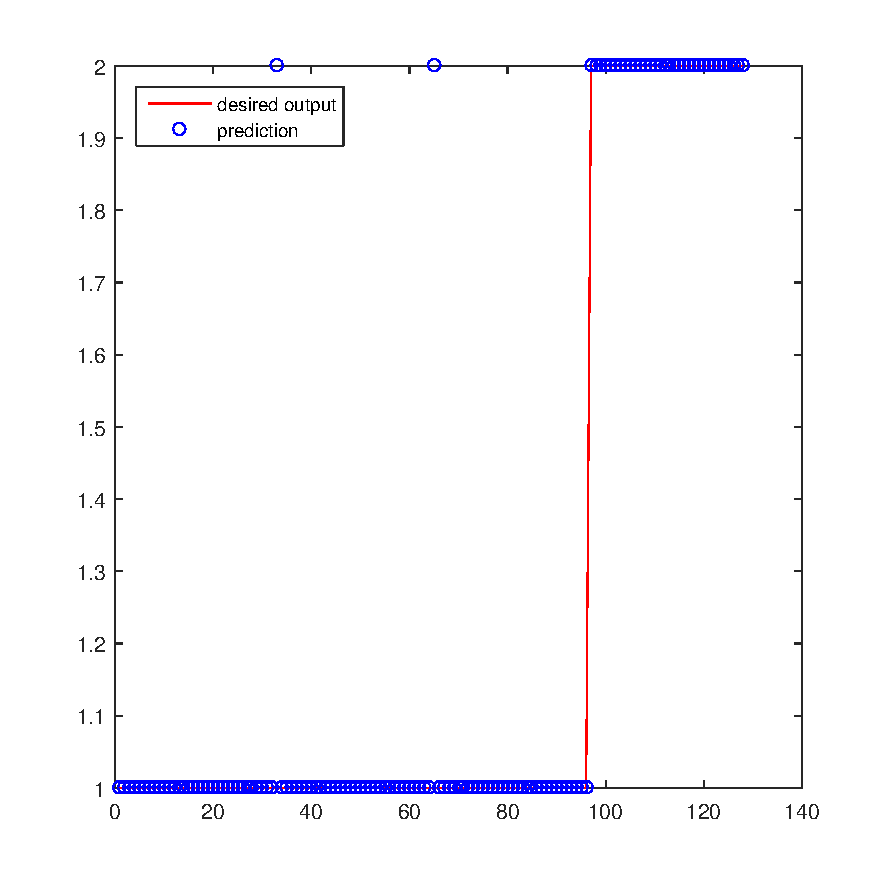
\includegraphics[scale=0.6]{breasths1}
			\newpage	
			\item accuracy = 98.4\%\ \\
			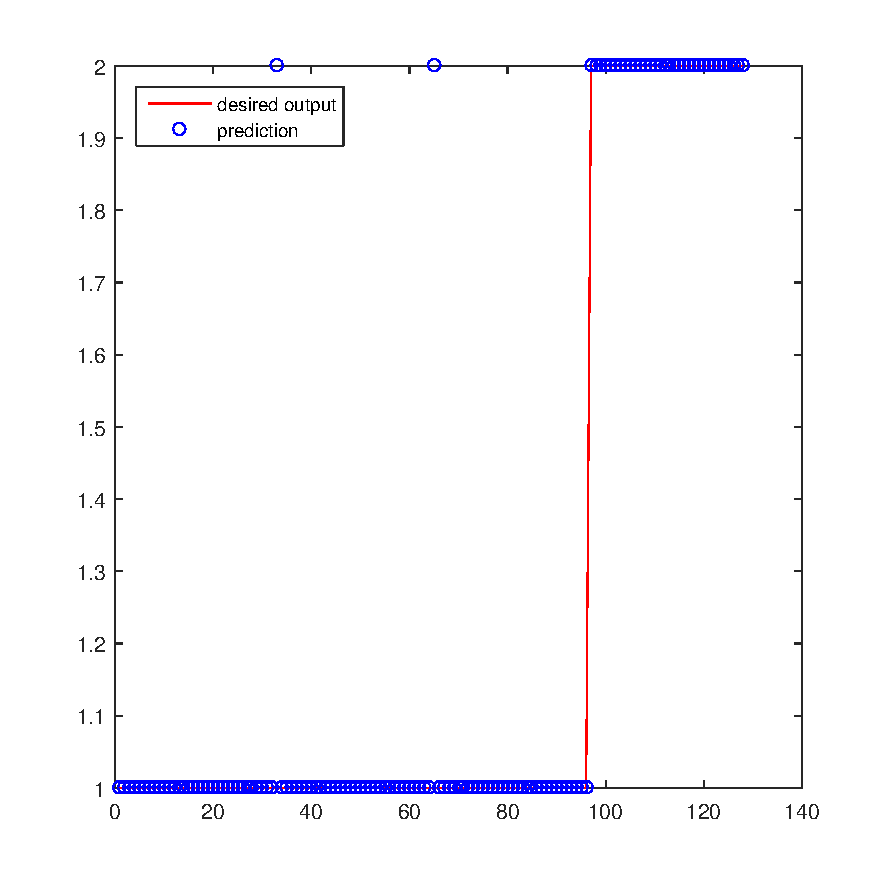
\includegraphics[scale=0.6]{breasths1}	
			\item accuracy = 98.4\%\ \\
			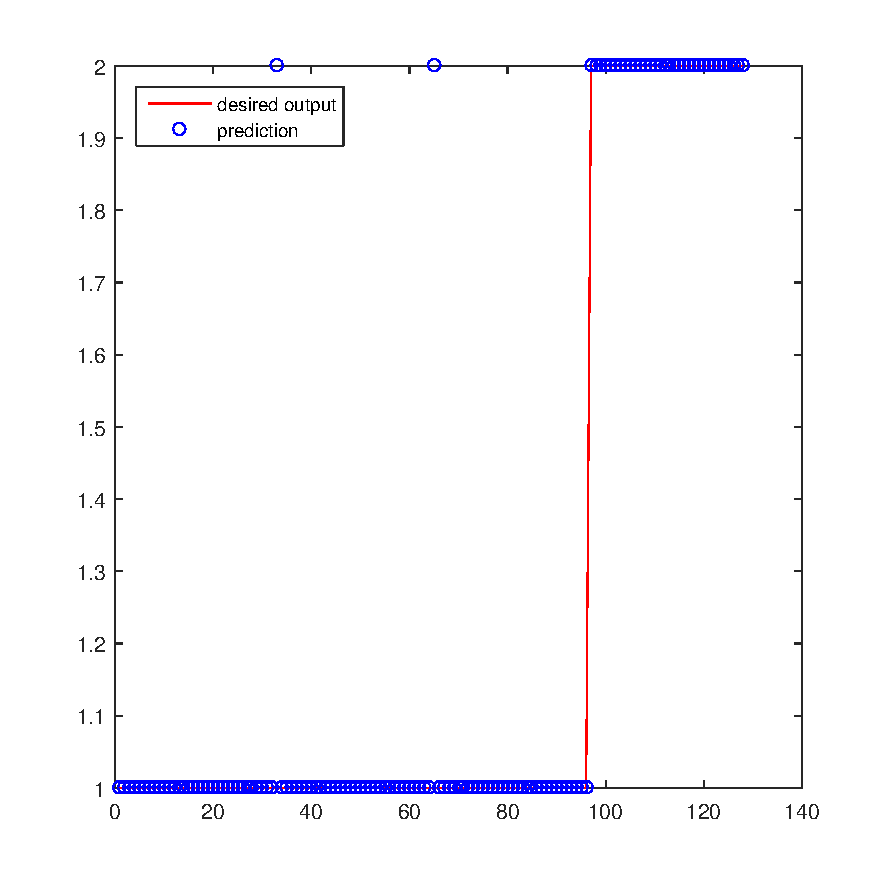
\includegraphics[scale=0.6]{breasths1}		
			\newpage	
		\end{enumerate}
	\end{enumerate}
	
	\item For the random weight assignment, use the same initial weights that you obtain the best classification result to compare the learning curves with different learning rates:
	\\
	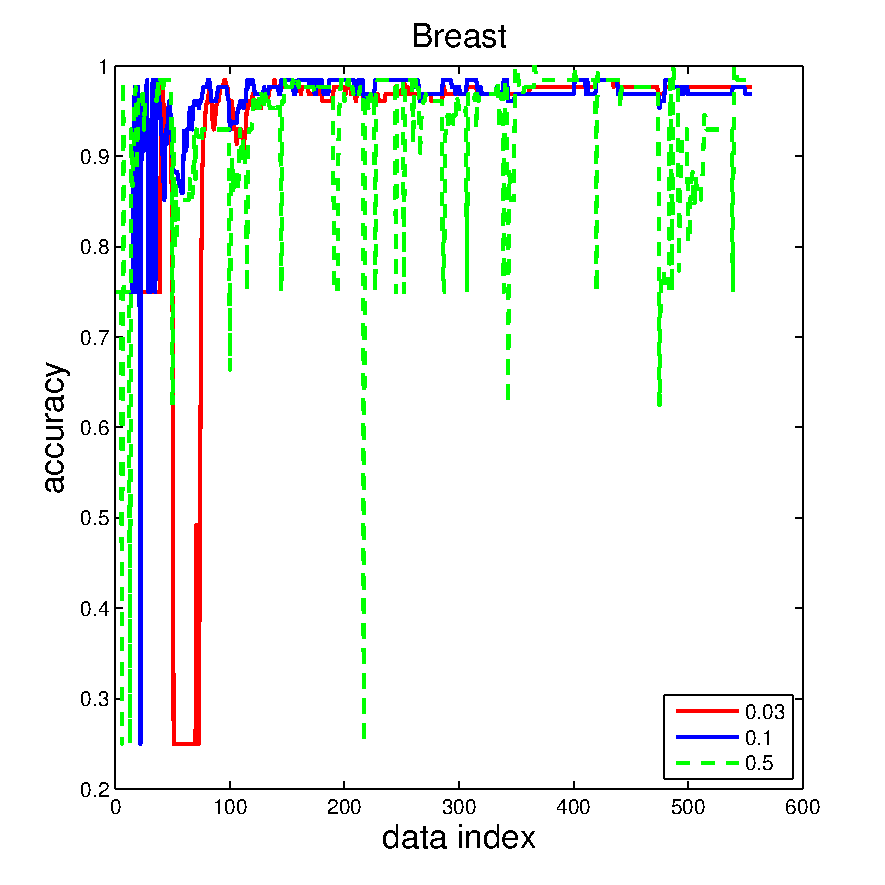
\includegraphics[scale=0.7]{breastcurve}

\end{enumerate}
\newpage
%%%%%%%%%%%%%%%%%%%%%%%%%%%%%%%%%%%%%%%%%%%%%
\item Yeast
\begin{enumerate}
	\item topologies (structures) of the networks: \\
	input layer node: 8 \\
	first hidden layer node: 5 \\
	second hidden layer node: 7 \\
	output layer node: 10\\
	all layers are fully connected
	\item best three results out of 10 trials using different initializations:
	\begin{enumerate}
		\item hyperbolic tangent functions for all the hidden layers:
		\\
		learning rate = 0.01 \\
		epoch = 500
		\begin{enumerate}
			\item accuracy = 59.7\%\\\
			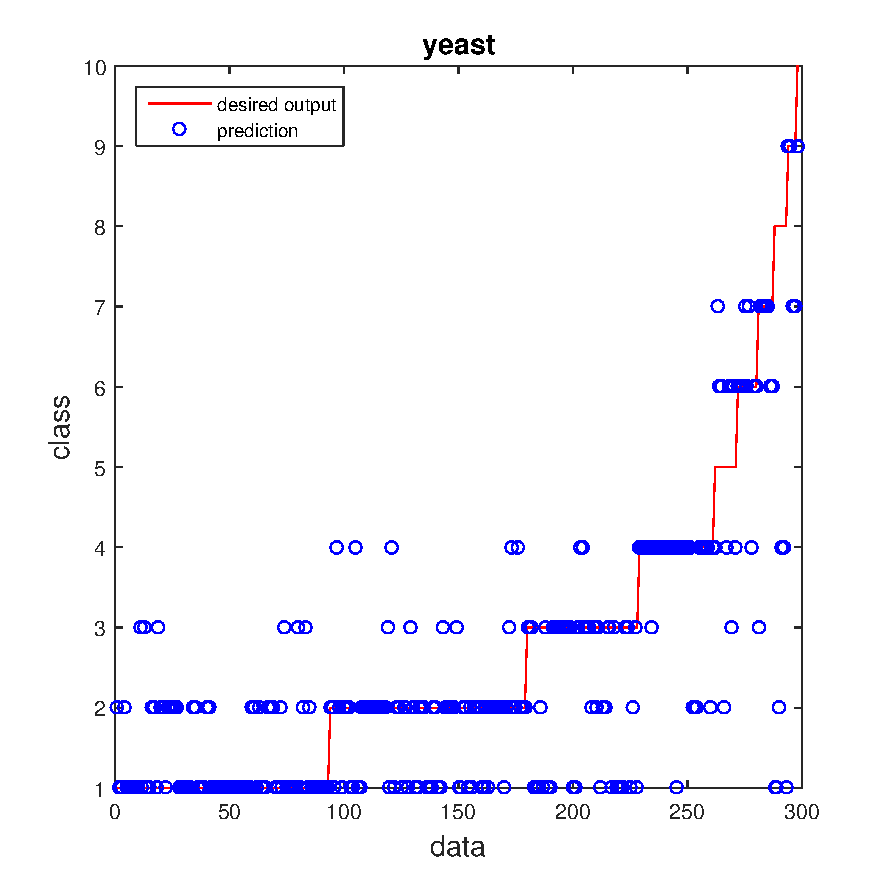
\includegraphics[scale=0.6]{yeasthh1}
			\newpage	
			\item accuracy = 58.4\%\\\
			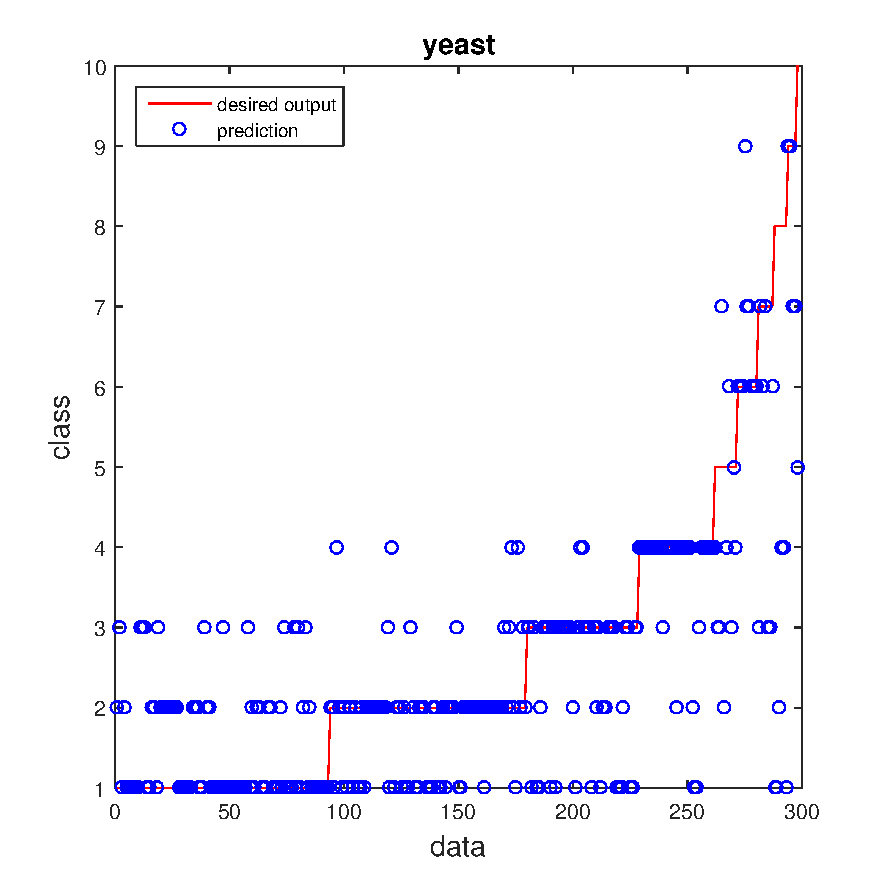
\includegraphics[scale=0.6]{yeasthh2}	
			\item accuracy = 58.1\%\\\
			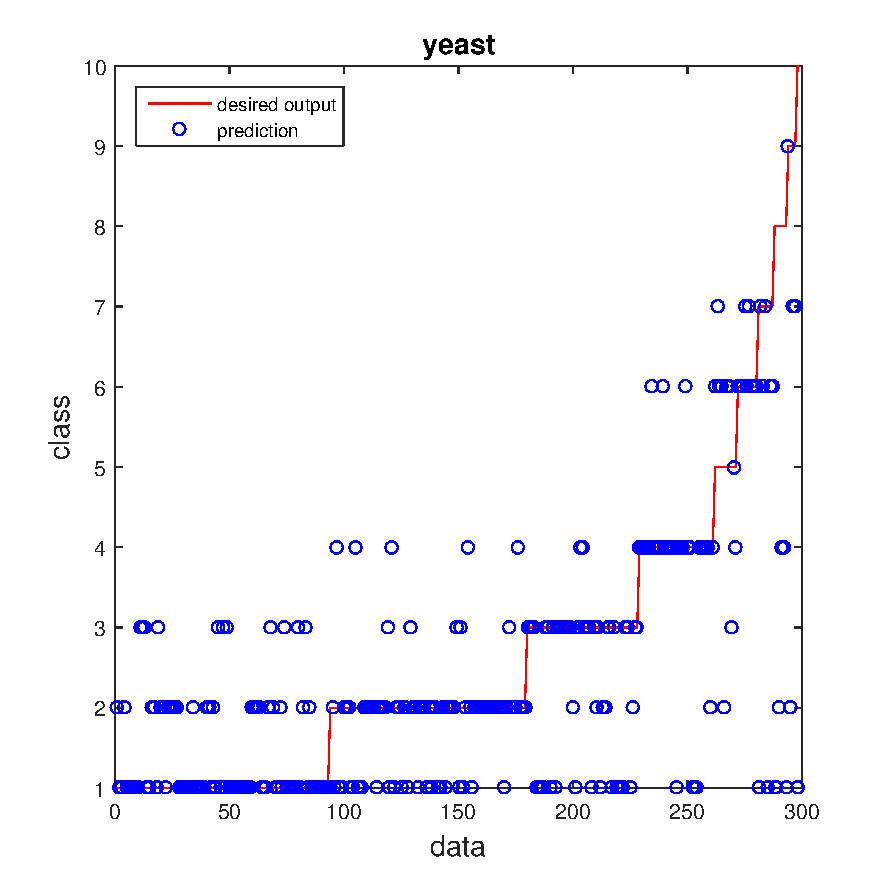
\includegraphics[scale=0.6]{yeasthh3}		
			\newpage	
		\end{enumerate}
		\item sigmoid functions for all the hidden layers:
		\\
		learning rate = 0.1 \\
		epoch = 500
		\begin{enumerate}
			\item accuracy = 58.1\%\ \\
			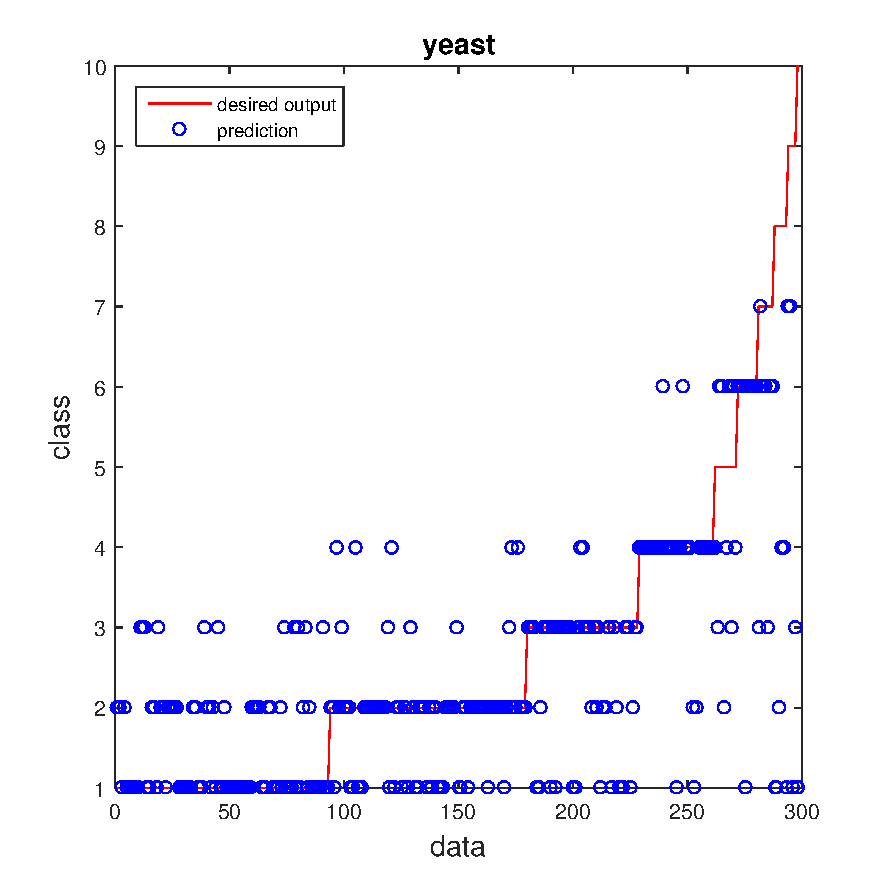
\includegraphics[scale=0.6]{yeastss1}
			\newpage	
			\item accuracy = 57.1\%\ \\
			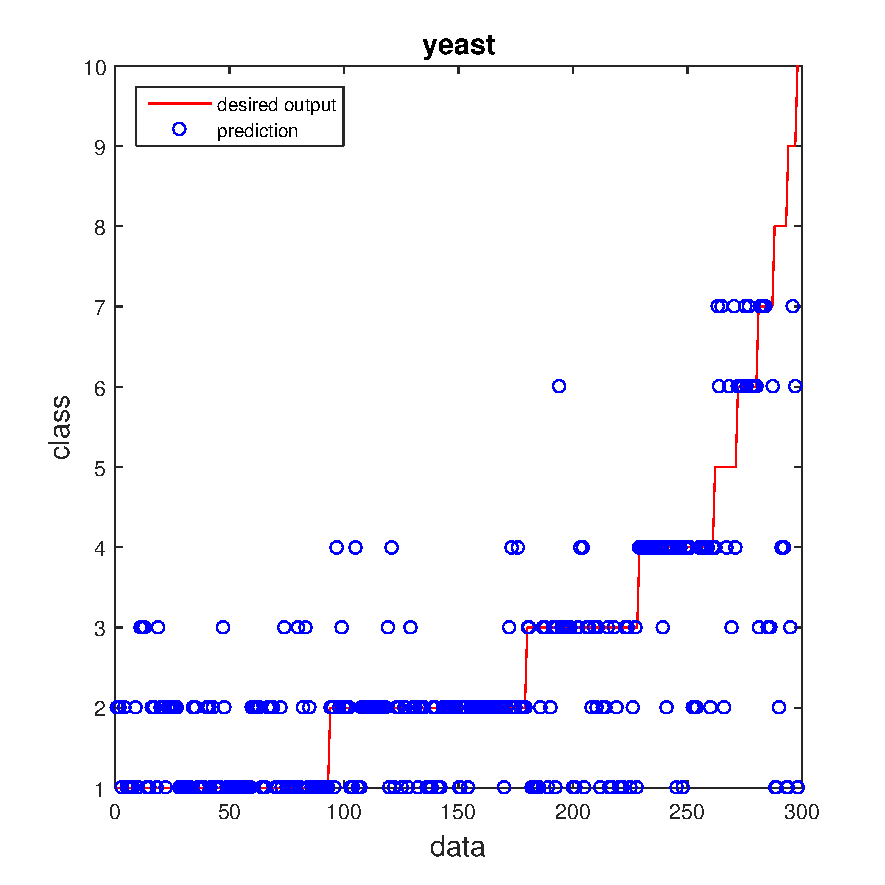
\includegraphics[scale=0.6]{yeastss2}	
			\item accuracy = 57.1\%\ \\
			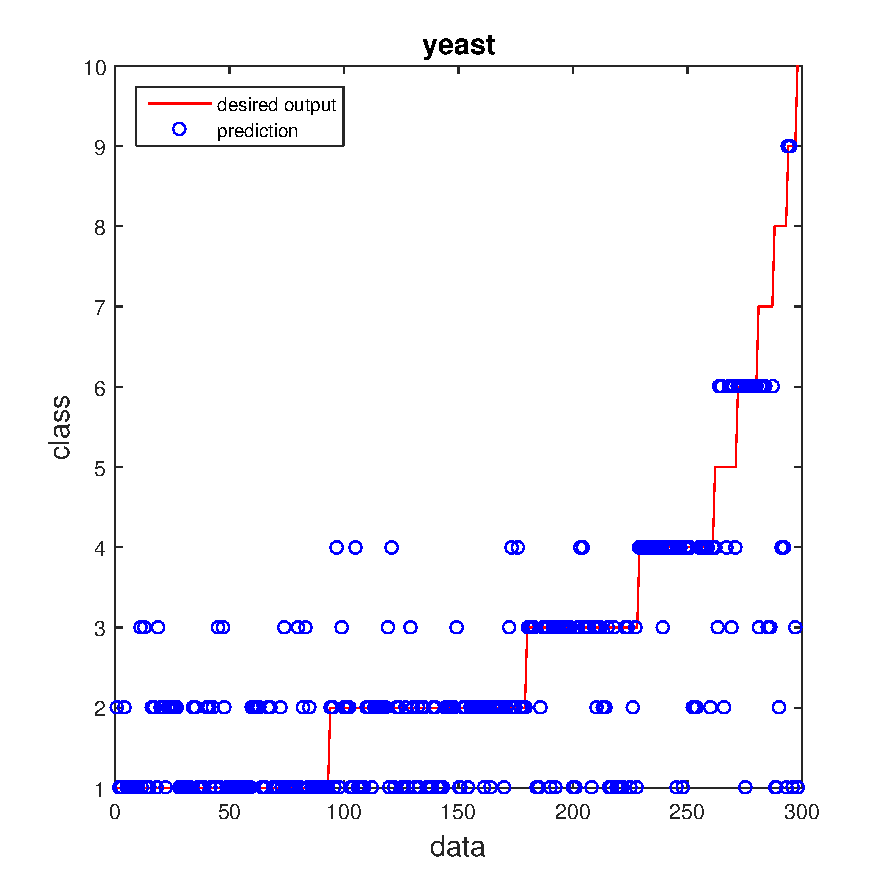
\includegraphics[scale=0.6]{yeastss3}		
			\newpage	
		\end{enumerate}
		\item hyperbolic tangent functions for the first hidden layer and sigmoid functions for the second layer:
		\\
		learning rate = 0.1 \\
		epoch = 500
		\begin{enumerate}
			\item accuracy = 58.4\%\ \\
			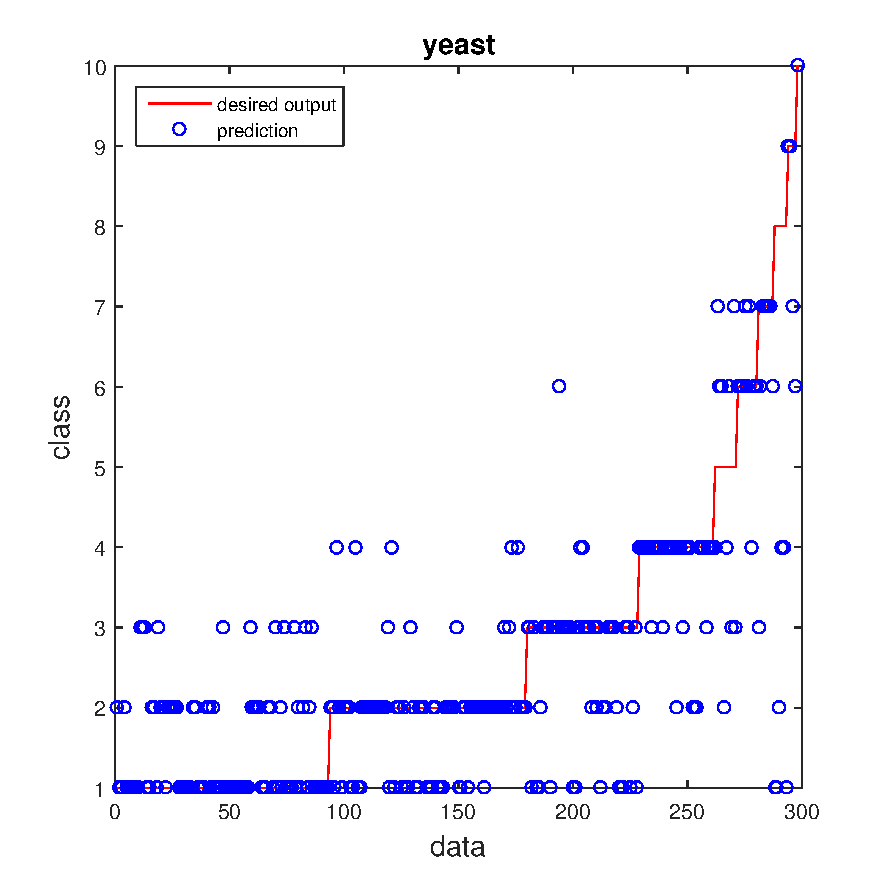
\includegraphics[scale=0.6]{yeasths1}
			\newpage	
			\item accuracy = 58.7\%\ \\
			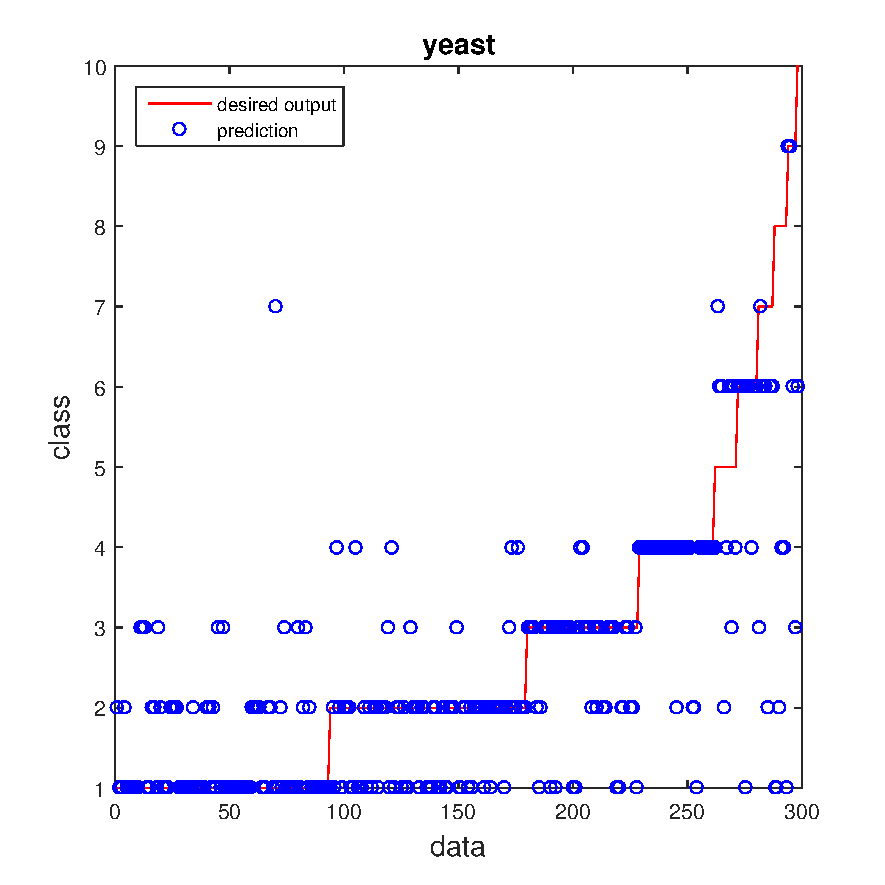
\includegraphics[scale=0.6]{yeasths2}	
			\item accuracy = 57.1\%\ \\
			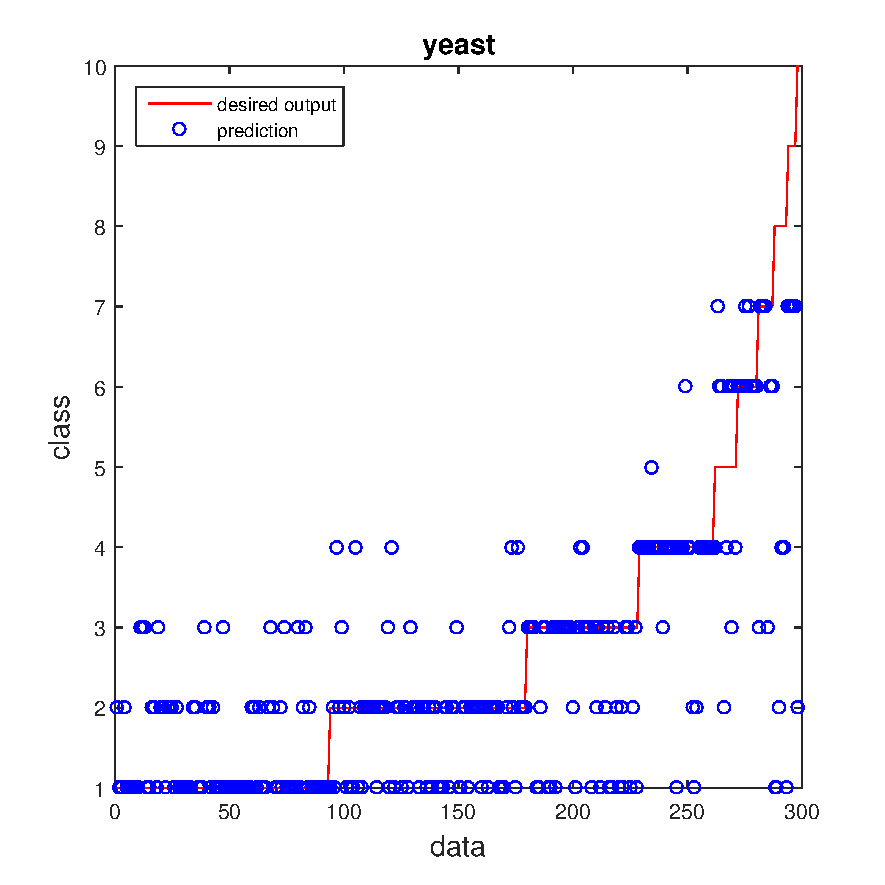
\includegraphics[scale=0.6]{yeasths3}		
			\newpage	
		\end{enumerate}
	\end{enumerate}
	
	\item For the random weight assignment, use the same initial weights that you obtain the best classification result to compare the learning curves with different learning rates:
	\\
	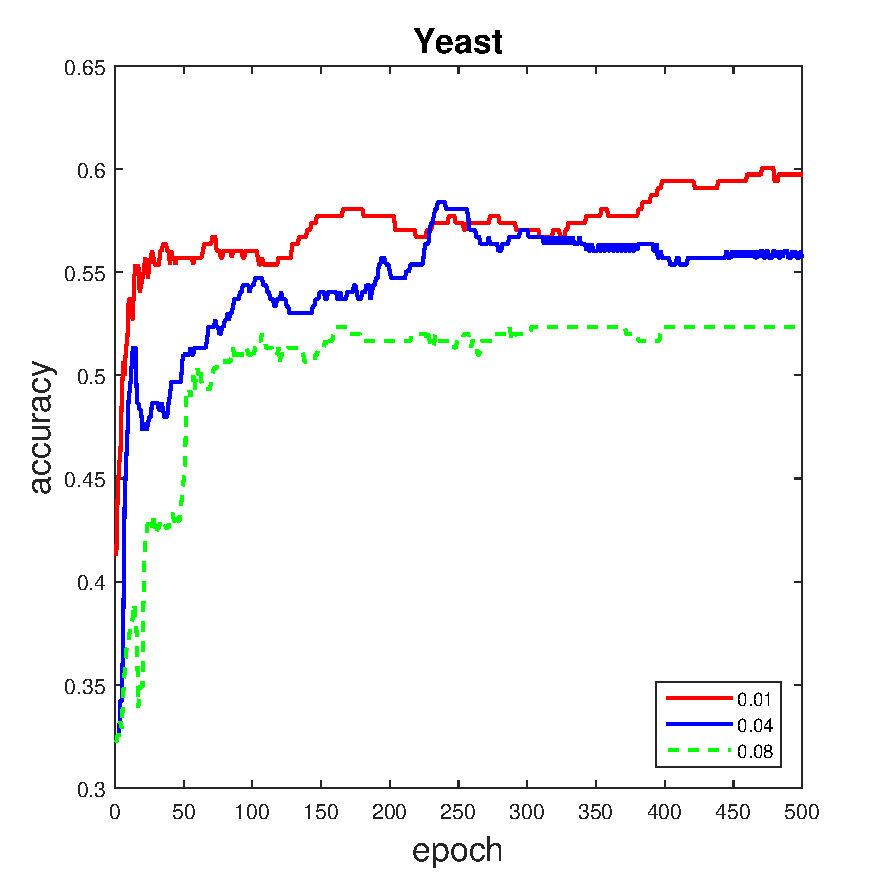
\includegraphics[scale=0.7]{yeastcurve}
	
\end{enumerate}
\end{enumerate}
%%%%%%%%%%%%%%%%%%%%%%%%%%%%%%%%%%%%%%%%%%%%%%
\newpage
\title{\large \bf  Part2: Function Approximation}
\\
	\begin{enumerate}
	\item topologies (structures) of the networks: \\
	input layer node: 2 \\
	first hidden layer node: 2 \\
	second hidden layer node: 3 \\
	output layer node: 2\\
	all layers are fully connected
	\item best three results out of 10 trials using different initializations:
	\\
	with learning rate =0.6, epoch =500
	\begin{enumerate}
	\item mean square errors $Y_1= 0.004 , Y_2=0.000448$ \\
	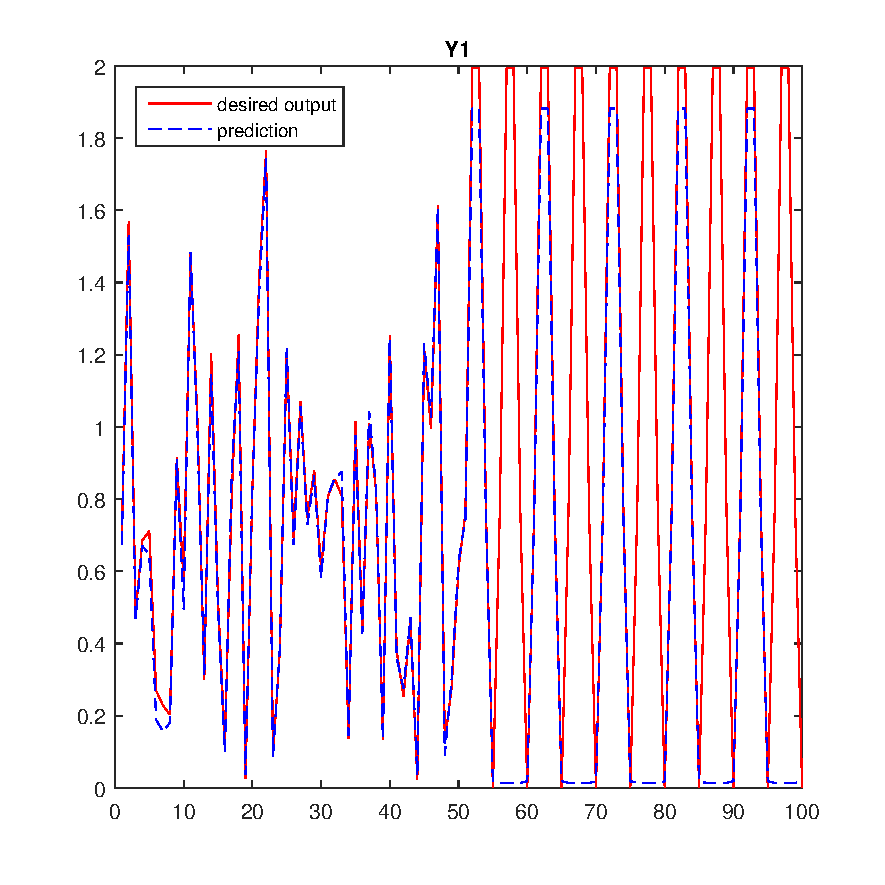
\includegraphics[scale=0.6]{y1} \\
	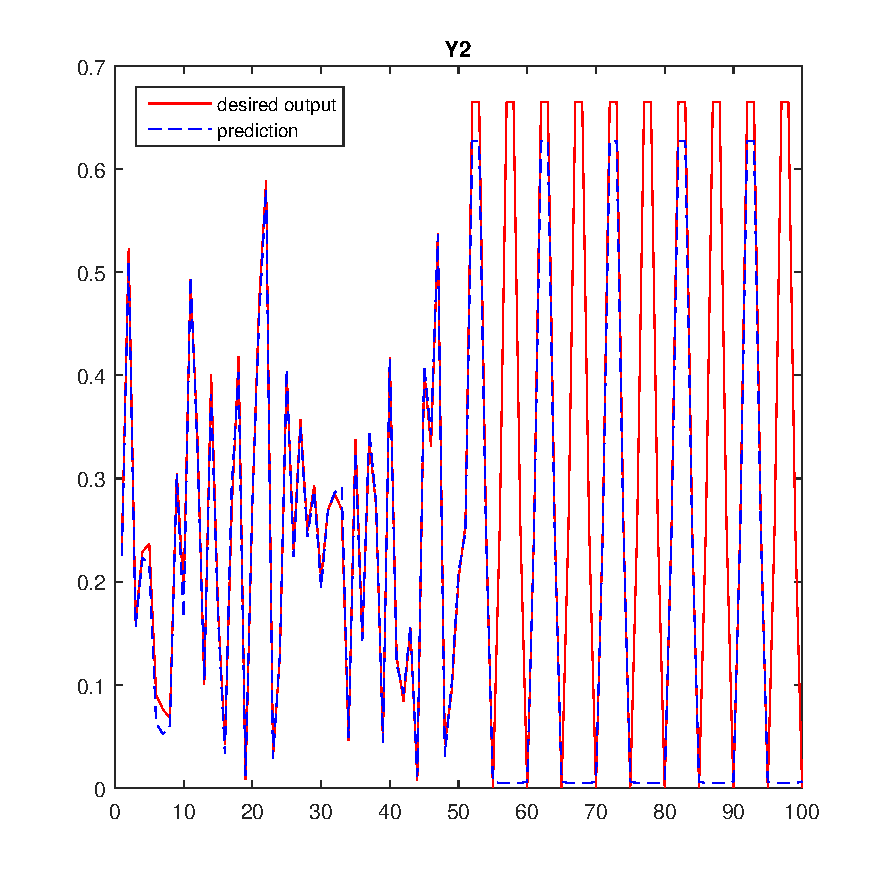
\includegraphics[scale=0.6]{y2}
	\newpage
	\item mean square errors $Y_1= 0.0041 , Y_2=0.000452$ \\
	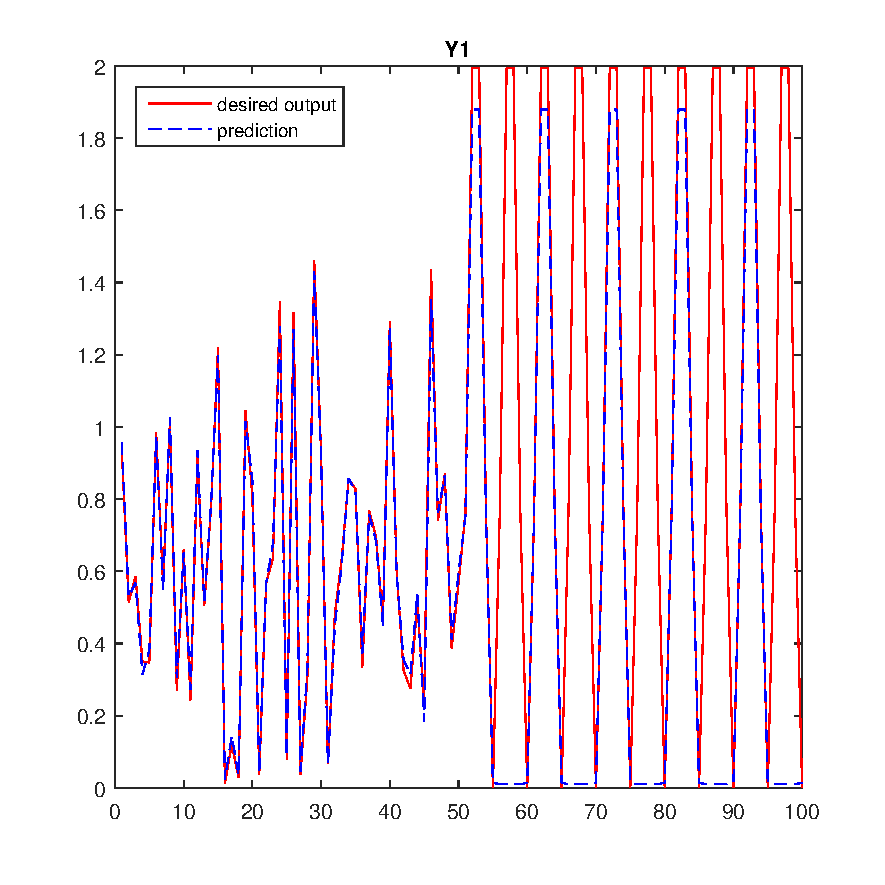
\includegraphics[scale=0.6]{y12} \\
	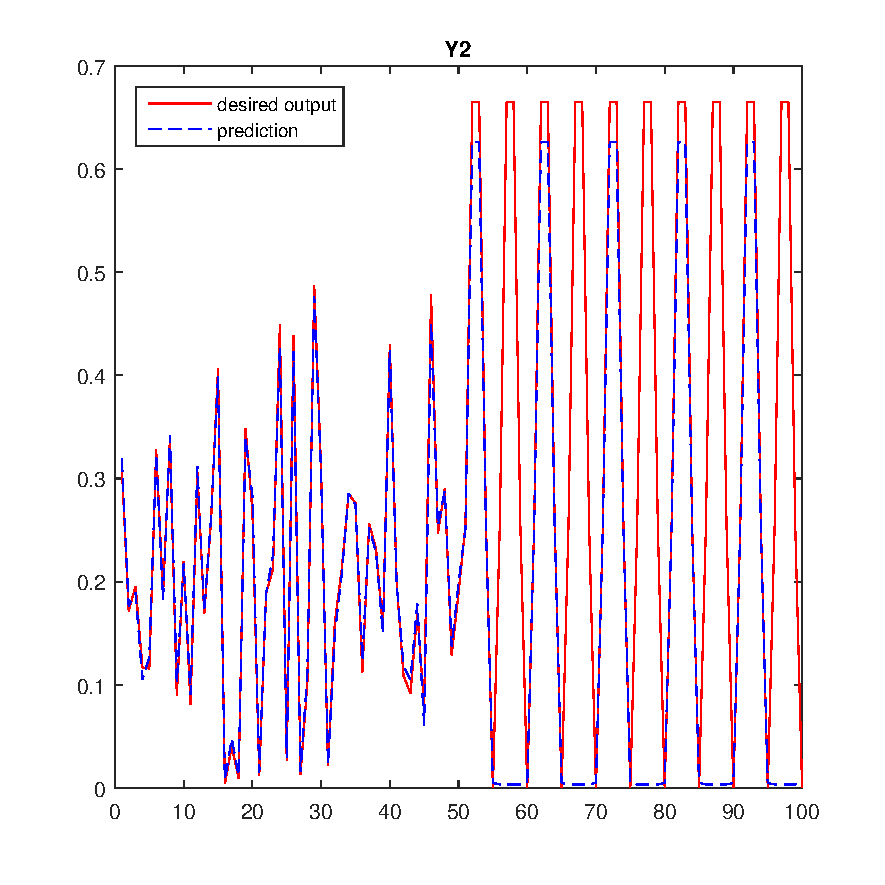
\includegraphics[scale=0.6]{y22}
	\newpage
	\item mean square errors $Y_1= 0.0041 , Y_2=0.000454$ \\
	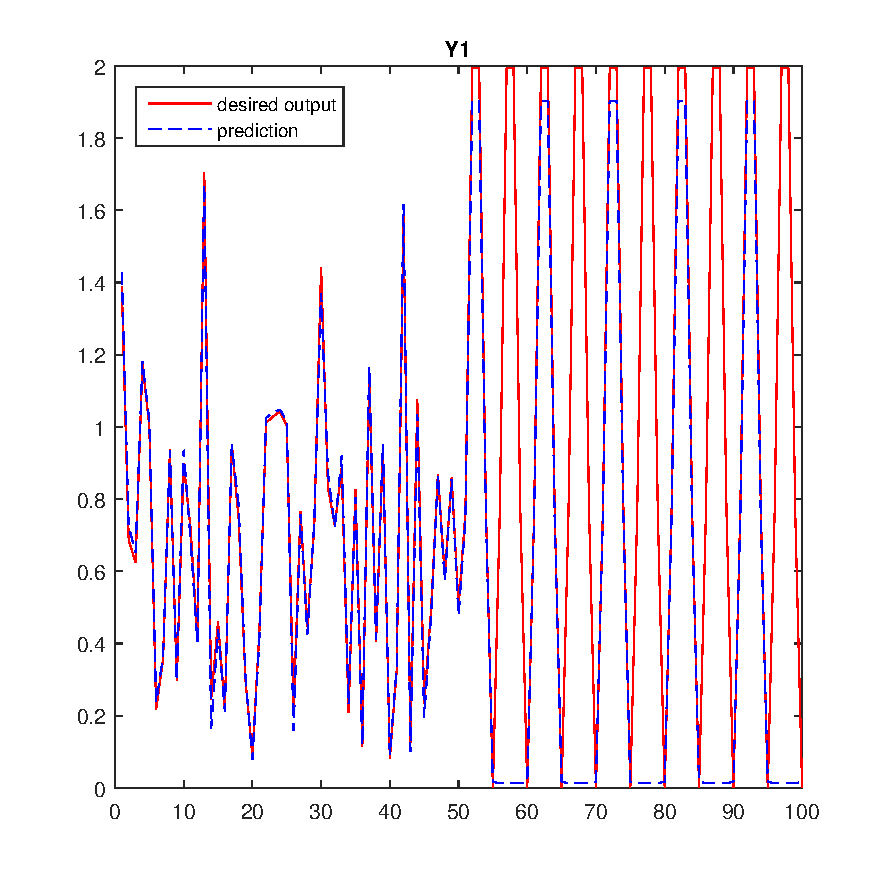
\includegraphics[scale=0.6]{y13} \\
	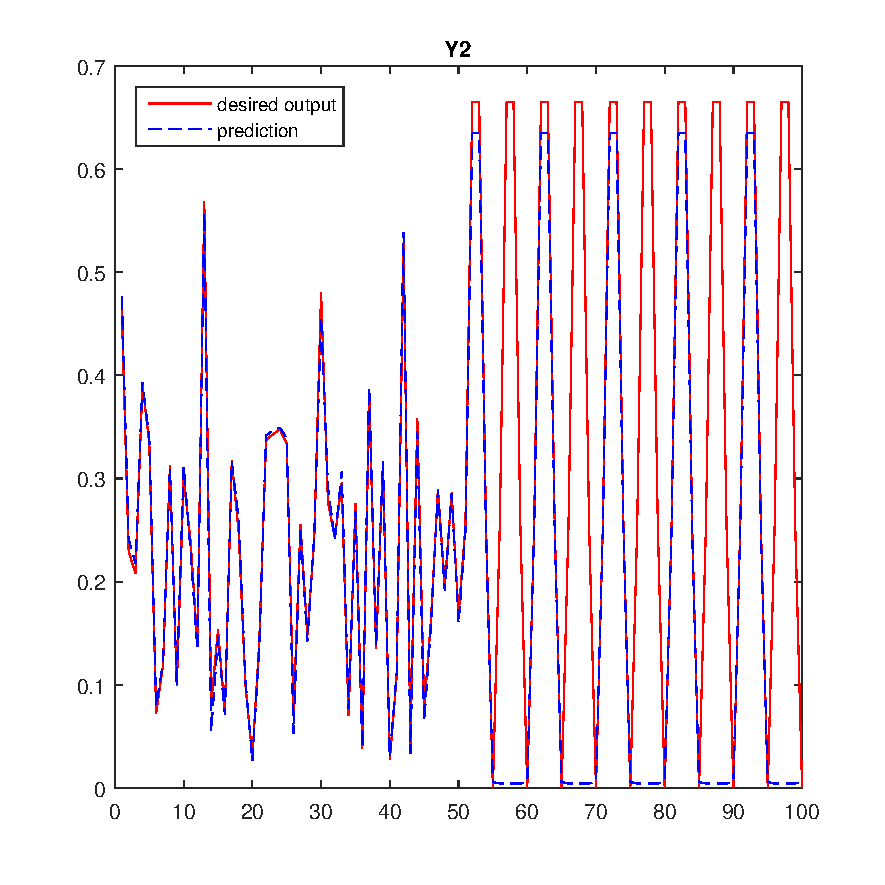
\includegraphics[scale=0.6]{y23}	
		
	\end{enumerate}
\newpage

\item For the random weight assignment, use the same initial weights that you obtain the best classification result to compare the learning curves with different learning rates:
\\
\\
learning rate of 0.03, 0.1, 0.6 are used
\\
	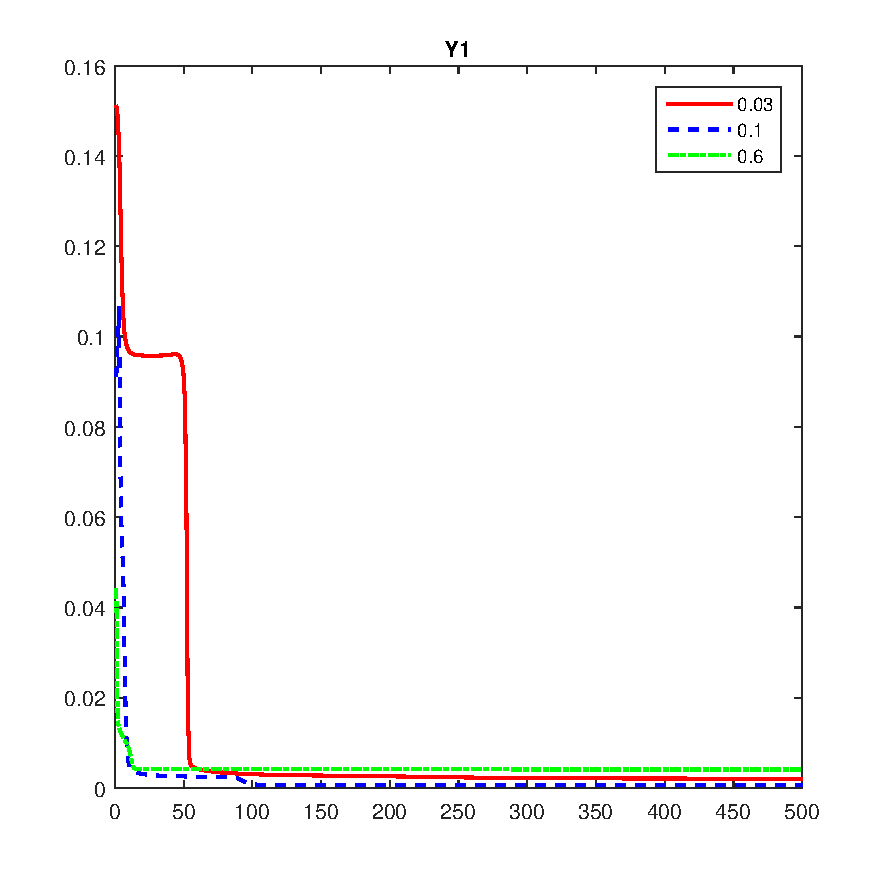
\includegraphics[scale=0.6]{y1curve}
	\\
	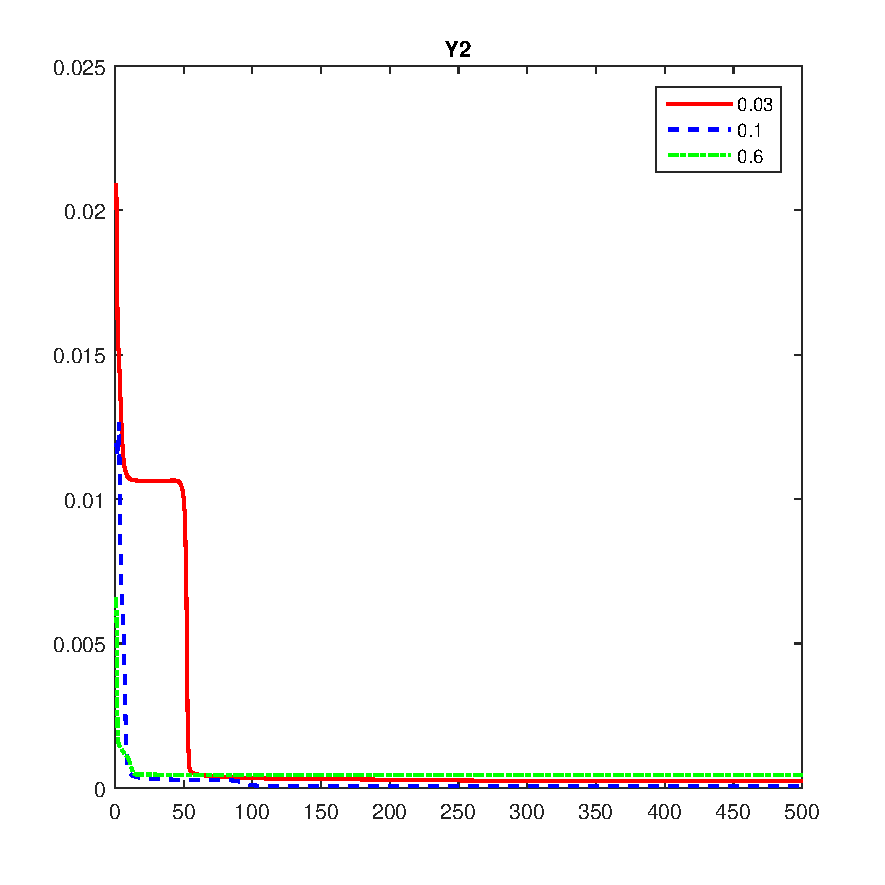
\includegraphics[scale=0.6]{y2curve}
	\end{enumerate}
\newpage
\title{\large \bf Discuss how to obtain a better result according to your experience in this homework:}
\\
To obtain a better result, learning rate, epoch, data sequence and the  number of nodes in the hidden layers are all important.
\begin{enumerate}
	\item learning rate: The lower the learning rate is, the better the result will be. But noted that the lower the learning rate is, the more epochs are needed to achieve the convergent result.
	\item epoch: For some data, a large number of epochs are needed to converge. Thus, it is better to have more epochs.
	\item data sequence: Sometimes, the training data are in an order. It is necessary to randomized the sequence of the training data. By doing this, the convergent time will descend.
	\item the number of nodes in the hidden layers: When dealing with simple classification or function approximation problem, nodes between 3 to 5 can provide good results than too many nodes or too little nodes.
\end{enumerate}
\end{CJK}

\end{document}